\chapter{Interferência}
\label{chpt:superp}
\textsl{{\sffamily(Versão: \today)}}

\noindent
Como a equação de onda~\eqref{eq:plweq3d} é linear (não inclui potências de
$\psi$ de grau superior a 1) e homogénea (não inclui potências de $\psi$ de grau
inferior a 1), as suas soluções satisfazem um princípio de sobreposição: a
combinação linear de duas soluções é também uma solução da equação de onda. Isto
significa que se num dado ponto do espaço coincidem duas ondas (da mesma
natureza, claro), então o valor da perturbação nesse ponto, num dado instante, é
a soma dos valores de cada uma das ondas, nesse ponto e nesse instante. No caso
das ondas eletromagnéticas, verifica\-\mbox{-se} que o campo elétrico e o campo
magnético resultantes da sobreposição de duas ondas são, em cada ponto e em cada
instante, respetivamente as somas dos campos elétricos e magnéticos das 
ondas que coincidem nesse ponto e nesse instante.

Neste capítulo vamos analisar a sobreposição de ondas e estudar alguns
fenómenos em que ela desempenha um papel importante. Os aspetos mais
interessantes da sobreposição de ondas são independentes da natureza específica
das ondas consideradas e, assim, são comuns às ondas de luz, de som, às ondas do
mar, etc.  Para demonstrar esses efeitos e ao mesmo tempo pôr em evidência a
simplicidade dos mecanismos físicos que os geram, começamos o capítulo com o
estudo da sobreposição de duas ondas sinusoidais unidimensionais com a mesma
frequência.  Em seguida, consideraremos a sobreposição de duas ondas planas
escalares arbitrárias, o que permite treinar as técnicas matemáticas da
sobreposição evitando ainda as complicações decorrentes da polarização.  Por
fim, já munidos de uma maior destreza matemática, repetiremos o estudo com ondas
com função de onda vetorial, como as ondas eletromagnéticas.

\section{Sobreposição de ondas 1D com iguais comprimento de onda e período}
\label{sec:sobrpos}
Sejam $\psi_1(x,t)$ e $\psi_2(x,t)$ duas ondas harmónicas com comprimento de
onda $\lambda$ e período $T$, que se propagam no sentido positivo do eixo dos
$x$, dadas por
\begin{align*}
\psi_1(x,t)&=A_1\cos\left(\Theta(x,t)+\varphi_1\right)&
\psi_2(x,t)&=A_2\cos\left(\Theta(x,t)+\varphi_2\right),
\end{align*}
onde, para aligeirar a notação, se introduziu o símbolo
$\Theta\equiv\Theta(x,t)=kx-\omega t,$ com $k=2\pi/\lambda$ e $\omega=2\pi/T$.
De acordo com o princípio da sobreposição, a resultante da sobreposição destas
duas ondas é uma onda com expressão geral
\begin{align*}
\psi(x,t)&=\psi_1(x,t)+\psi_2(x,t)\\
&=A_1\cos(\Theta+\varphi_1)+A_2\cos(\Theta+\varphi_2)
\end{align*}
Usando aqui a igualdade trigonométrica
$\cos(\alpha+\beta)=\cos\alpha\cos\beta-\sin\alpha\sin\beta$, esta expressão
pode reescrever-se como
\begin{equation*}
\psi(x,t)=(A_1\cos\varphi_1+A_2\cos\varphi_2)\cos\Theta-
(A_1\sin\varphi_1+A_2\sin\varphi_2)\sin\Theta.
\end{equation*}
Introduzimos agora dois números reais, $A$ e $\varphi$, definidos como
\begin{align*}
A\cos\varphi&=A_1\cos\varphi_1+A_2\cos\varphi_2\\
A\sin\varphi&=A_1\sin\varphi_1+A_2\sin\varphi_2.
\end{align*}
Substituindo acima e invocando de novo a igualdade trigonométrica para o cosseno
da soma de dois ângulos já usada, obtemos
\begin{equation}
\psi(x,t)=A\cos\left(\Theta+\varphi\right)=
A\cos\left(kx-\omega t+\varphi\right).
\end{equation}
Assim, concluímos que a sobreposição de duas ondas harmónicas com iguais período
e comprimento de onda é ainda uma onda harmónica, com o mesmo período e com o
mesmo comprimento de onda, com amplitude e constante de fase que dependem das
amplitudes e das constantes de fase de cada uma das ondas que se sobrepõem.

Os números reais $A$ e $\varphi$ (a amplitude e a constante de fase da onda
resultante) satisfazem as equações
\begin{align*}
A\cos\varphi&=A_1\cos\varphi_1+A_2\cos\varphi_2\\
A\sin\varphi&=A_1\sin\varphi_1+A_2\sin\varphi_2.
\end{align*}
Elevando estas duas equações ao quadrado, somando os resultados e usando a
igualdade fundamental da trigonometria, obtemos para $A$ a expressão
\begin{equation}
A^2=A_1^2 +
  A_2^2 + 2A_1A_2(\cos\varphi_1\cos\varphi_2+\sin\varphi_1\sin\varphi_2)
\end{equation}
Mas a combinação entre parentesis é igual a $\cos(\varphi_1-\varphi_2)$, que é a
diferença de fase das duas ondas. A amplitude da sobreposição pode então
escrever-se como\footnote{Já agora, é fácil nesta altura demonstrar que a
quantidade real $A$ existe mesmo (até aqui, apenas podíamos garantir que $A^2$
existe. Mas, se acontecer $A^2<0$, então $A$ não pode ser real.) Com efeito, uma
vez que $\cos\delta\varphi=\cos(\varphi_1-\varphi_2)\geq-1$, segue-se que
$A_1^2+A_2^2+2A_1A_2\cos\delta\varphi\geq A_1^2+A_2^2-2A_1A_2=(A_1-A_2)^2\geq
0$. Logo, $A^2\geq0$, ou seja, $A\in
\mathbb{R}$.}
\begin{equation}
A=\sqrt{A_1^2+A_2^2+2A_1A_2\cos\delta\varphi},\qquad
\delta\varphi=\varphi_1-\varphi_2.
\end{equation}
%
A constante de fase da onda resultante pode agora também ser facilmente
calculada através de
\begin{align}
\cos\varphi&=\frac{A_1\cos\varphi_1+A_2\cos\varphi_2}{A}&
\sin\varphi&=\frac{A_1\sin\varphi_1+A_2\sin\varphi_2}{A}.
\end{align}

\subsection{Interferência construtiva e destrutiva}
\label{sec:condint}
Em virtualmente todas as situações com interesse físico, a potência transportada
pela onda é proporcional ao quadrado da sua amplitude (já o vimos para o caso
das ondas eletromagnéticas, na Secção~\ref{sec:irradiance}). Representando a
constante desta proporcionalidade por $\alpha$, temos então
\begin{align}
I=\alpha A^2&=\alpha A_1^2+\alpha A_2^2 + 2\alpha A_1 A_2\cos\delta\varphi
\nonumber\\
&=I_1+I_2+2\sqrt{I_1I_2}\cos\delta\varphi.\label{eq:superp1}
\end{align}
A intensidade da onda resultante da sobreposição de duas ondas é então igual à
soma das suas intensidades, mais uma contribuição dita de \emph{interferência.}
Como o termo de interferência pode ser positivo ou negativo, em função do valor
do cosseno da diferença de fases, a intensidade da sobreposição pode ser maior
ou menor do que a soma das intensidades das duas ondas que se sobrepõem.  Quando
se verifica a primeira possibilidade, falamos de \emph{interferência
construtiva;} quando se dá o segundo, de \emph{interferência destrutiva.}
Chamam especial atenção os dois casos extremos, particularmente interessantes:
\begin{itemize}
\item \textbf{Interferência totalmente construtiva}\\
Quando a diferença entre as fases das duas ondas é um múltiplo inteiro de $2\pi$,
isto é, quando
\begin{equation*}
\delta\varphi = 2l\pi,\quad l=0,\pm1,\pm2,\ldots,
\end{equation*}
dizemos que as duas ondas que se sobrepõem estão \emph{em fase.} Nestas
condições, $\cos\delta\varphi=1$, e assim a intensidade da sobreposição resulta
\begin{equation*}
I=I_1 + I_2+2\sqrt{I_1I_2}.
\end{equation*}
Nesta situação o reforço da intensidade das duas ondas é máximo. Se as duas ondas
tiverem intensidades iguais $I_0$, a intensidade da resultante será $4I_0$, ou
seja duas vezes maior do que a soma das intensidades das duas ondas.
\item \textbf{Interferência totalmente destrutiva}\\
Quando a diferença entre as fases das duas ondas é um múltiplo semi-inteiro de
$2\pi$, ou seja, quando
\begin{equation*}
\delta\varphi = 2\left(l\pm\frac{1}{2}\right)\pi,\quad l=0,\pm1,\pm2,\ldots,
\end{equation*}
dizemos que as duas ondas estão em \emph{oposição de fase.} Agora temos
$\cos\delta\varphi=-1$ e obtemos para a intensidade da sobreposição
\begin{equation*}
I=I_1 + I_2 - 2\sqrt{I_1I_2}
\end{equation*}
Agora é máxima a atenuação da intensidade da sobreposição. De facto, se as duas
ondas tiverem intensidades iguais, a intensidade da resultante é nula!
\end{itemize}
A Figura~\ref{fig:icd} ilustra estes dois casos extremos de sobreposição de ondas
unidimensionais harmónicas com igual frequência e comprimento de onda.
\begin{figure}[htb]
  {\centering
    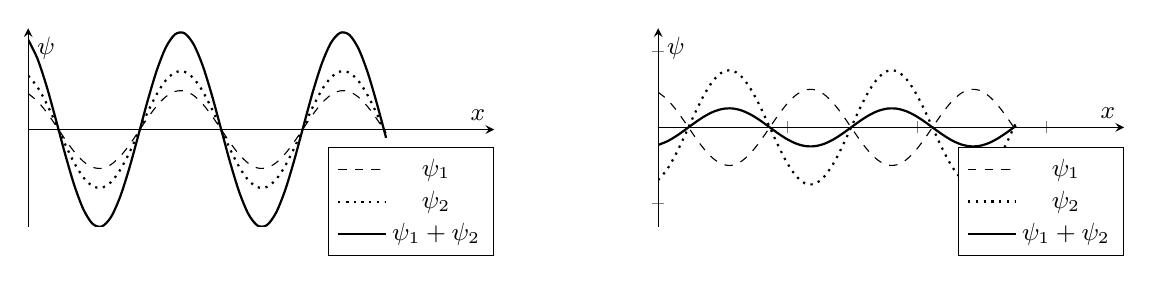
\begin{tikzpicture}
      \small
      \begin{scope}[xshift=-4.0cm]
      \begin{axis}[domain=0:4.4*pi,samples=40,xmax=18,ymax=2.6,
        legend style={at={(1,0.4)}},ylabel=$\psi$,
        xlabel=$x$,height=4.1cm,width=7.5cm,
        axis lines=middle,ticks=none,
        xticklabels={},yticklabels={}]
        \addplot [dashed, mark=none,smooth] {cos(deg(x+0.4))};
        \addplot [thick, dotted,mark=none,smooth] {1.5*cos(deg(x+0.4))};
        \addplot [thick,mark=none,smooth] {2.5*cos(deg(x+0.4))};
        \legend{$\psi_1$,$\psi_2$, $\psi_1+\psi_2$}
      \end{axis}
      \end{scope}
      \begin{scope}[xshift=4.0cm]
      \begin{axis}[domain=0:4.4*pi,samples=40,xmax=18,ymax=2.6,ymin=-2.6,
        legend style={at={(1,0.4)}},ylabel=$\psi$,
        xlabel=$x$,height=4.1cm,width=7.5cm,
        axis lines=middle,
        xticklabels={},yticklabels={}]
        \addplot [dashed, mark=none,smooth] {cos(deg(x+0.4))};
        \addplot [thick, dotted,mark=none,smooth] {-1.5*cos(deg(x+0.4))};
        \addplot [thick,mark=none,smooth] {-0.5*cos(deg(x+0.4))};
        \legend{$\psi_1$,$\psi_2$, $\psi_1+\psi_2$}
      \end{axis}
      \end{scope}
    \end{tikzpicture}\par
  }
  \caption{Interferência totalmente construtiva (à esquerda) e interferência
  totalmente destrutiva (à direita) de duas ondas $\psi_1$ e $\psi_2$ com igual
  frequência e comprimento de onda.\label{fig:icd}}
\end{figure}

Vimos na Secção~\ref{sec:hamonicwaves} que o valor da constante de fase de uma
onda é, no essencial, fixado por nós arbitrariamente, já que depende da escolha
que fazemos para a posição da origem do sistema de coordenadas e para o instante
que consideramos inicial.  Nessa medida, a constante de fase parece não ter um
significado físico muito relevante. É verdade, mas o mesmo não se pode dizer da
\emph{diferença de fase} de duas ondas (e, se elas tiverem o mesmo comprimento
de onda e a mesma frequência, essa diferença é igual à diferença entre as suas
constantes de fase). Como acabámos de constatar, o resultado da sobreposição de
duas ondas depende dramaticamente da diferença entre as suas fases. Ou seja, a
diferença entre as duas irrelevâncias é muitíssimo relevante: determina a
intensidade da sobreposição das duas ondas.


\section{Sobreposição de ondas escalares 3D}\label{sec:scalarsuperp}
Agora que estudámos a sobreposição de ondas no caso mais simples (ondas
unidimensionais com iguais frequências e comprimentos de onda), vamos abordar o
mesmo problema de forma mais geral, considerando ondas com frequências e
comprimentos de onda não necessariamente iguais no espaço normal tridimensional.

Consideremos duas ondas planas sinusoidais 3D com função de onda escalar
$\psi_1(\vec r,t)$ e $\psi_2(\vec r,t)$, com frequências $\omega_1$ e $\omega_2$
e vetores de onda $\vec k_1$ e $\vec k_2$, definidas numa mesma região do
espaço.  Estas ondas não são (nem pretendem ser) ondas de luz, que têm função de
onda vetorial mas, se pretendemos com esta análise extrair conclusões aplicáveis
à luz, $\psi_1$ e $\psi_2$ devem partilhar o maior número posssível das
características da luz. São funções escalares, porque assim o queremos para
simplificar os cálculos mas, em tudo o resto, devem semelhantes às ondas de luz.
Em particular, a frequência, o comprimento de onda e o módulo da amplitude devem
ter os valores típicos das ondas de luz. Suponhamos que a intensidade destas
ondas é, como a das ondas eletromagnéticas (ver a Secção~\ref{sec:irradiance}),
proporcional à média temporal, tomada ao longo de um intervalo de tempo com
duração razoável\footnote{Por \emph{duração razoável} deve entender-se a
necessária para se fazer uma observação. Como as ondas de luz têm frequências
muito altas, as operações de medida ou de observação têm sempre uma duração
muito maior do que o período das oscilações da função de onda.  Assim, deve
considerar-se \emph{duração razoável} a de qualquer intervalo de tempo muito
maior que o período das funções $\psi_1$ e $\psi_2$.} $[0,\,\tau],\ \tau>>T$, do
quadrado da função de onda,
\begin{equation*}
I=\alpha \langle \psi^2\rangle_\tau,
\end{equation*}
onde $\alpha$ é alguma constante característica das ondas consideradas e
\begin{equation*}
\langle X\rangle_\tau =\frac{1}{\tau}\int_0^\tau X\,dt
\end{equation*}
representa a média temporal da função $X$ no intervalo de tempo $[0,\,\tau]$.
Assim, temos
\begin{align*}
I_1&=\alpha\langle\psi_1^2\rangle_\tau&
I_2&=\alpha\langle\psi_2^2\rangle_\tau,
\end{align*}
e, claro está,
\begin{align}
I&=\alpha\langle\psi^2\rangle_\tau=
  \alpha\langle(\psi_1+\psi_2)^2\rangle_\tau\nonumber\\
&=I_1+I_2+I_{12},\label{eq:superp2}
\end{align}
onde
\begin{equation*}
I_{12}=2\alpha\langle\psi_1\psi_2\rangle_\tau.
\end{equation*}
Assim, e à semelhança do que verificámos no estudo mais simplificado da
Secção~\ref{sec:sobrpos}, a intensidade da onda resultante da sobreposição de
$\psi_1$ e $\psi_2$ não é em geral apenas a soma das intensidades de cada uma,
há ainda uma contribuição adicional, dita de \emph{interferência,} traduzida
pelo termo $I_{12}$. Este termo de interferência pode ser positivo ou negativo;
logo, a intensidade da onda resultante pode ser maior ou menor do que a soma das
intensidades das ondas que se sobrepõem. Em geral, estas duas possibilidades
ocorrem em simultâneo, verificando-se um reforço da intensidade nuns pontos e
uma atenuação noutros. 

Podemos explicitar melhor o termo de interferência atribuindo expressões
concretas para as duas ondas que se sobrepõem. Por hipótese, temos estado a
considerar ondas planas sinusoidais; então,
\begin{align*}
\psi_1(\vec r,t)&=A_1\cos\left(\vec k_1\cdot\vec r-\omega_1 t+\varphi_1\right)&
\psi_2(\vec r,t)&=A_2\cos\left(\vec k_2\cdot\vec r-\omega_2 t+\varphi_2\right).
\end{align*}
Para aliviar a notação, introduzam-se as funções da posição $\phi_i=\phi_i(\vec
r)=\vec k_i\cdot r+\varphi_i,\ i=1,2$. Substituindo estas expressões de
$\psi_1$, $\psi_2$ na expressão do termo de interferência e usando a seguir a
igualdade trignométrica elementar
$\cos(\alpha+\beta)=\cos\alpha\cos\beta-\sin\alpha\sin\beta$, resulta
\begin{align}
I_{12}&=2\alpha A_1A_2
  \langle\cos(\phi_1-\omega_1t)\cos(\phi_2-\omega_2t)\rangle_\tau\nonumber\\
  &=2\alpha A_1A_2 \left\langle
    (\cos\phi_1\cos\omega_1t+\sin\phi_1\sin\omega_1t)
    (\cos\phi_2\cos\omega_2t+\sin\phi_2\sin\omega_2t)
  \right\rangle_\tau\nonumber\\
&=2\alpha A_1A_2 \left\{
    \cos\phi_1\cos\phi_2\langle\cos\omega_1t\cos\omega_2t\rangle_\tau+
    \cos\phi_1\sin\phi_2\langle\cos\omega_1t\sin\omega_2t\rangle_\tau+\right.
    \nonumber\\
&\hspace{2cm}\left.
    \sin\phi_1\cos\phi_2\langle\sin\omega_1t\cos\omega_2t\rangle_\tau+
    \sin\phi_1\sin\phi_2\langle\sin\omega_1t\sin\omega_2t\rangle_\tau\right\}
    \label{eq:i12}
\end{align}
Devemos agora estimar o valor das quatro médias temporais no lado direito desta
igualdade. Tenha presente que, por hipótese, o intervalo de tempo considerado
para estas médias tem uma duração $\tau$ muito maior do que o período de
qualquer das ondas $\psi_1$ e $\psi_2$. Note também que as funções do tempo
cujas médias queremos calcular são o produto de duas funções seno e/ou cosseno.
Ora, os produtos destas funções podem escrever-se como médias aritméticas de
funções seno e cosseno, de acordo com as igualdadades trignométricas elementares
seguintes:
\begin{align*}
\cos\alpha\cos\beta&=\frac{1}{2}
    \left[\cos(\alpha+\beta)+\cos(\alpha-\beta)\right]\\
\sin\alpha\sin\beta&=-\frac{1}{2}
    \left[\cos(\alpha+\beta)-\cos(\alpha-\beta)\right]\\
\sin\alpha\cos\beta&=\frac{1}{2}
    \left[\sin(\alpha+\beta)+\sin(\alpha-\beta)\right]
\end{align*}
Assim sendo, tomando por exemplo a primeira das médias na eq.~\eqref{eq:i12},
temos
\begin{equation*}
\langle\cos\omega_1t\cos\omega_2t\rangle_\tau=
\frac{1}{2}\langle\cos(\omega_1+\omega_2)t\rangle_\tau+
\frac{1}{2}\langle\cos(\omega_1-\omega_2)t\rangle_\tau.
\end{equation*}
A primeira média no lado direito desta igualdade tem um valor desprezável,
porque o cosseno é uma função que realiza oscilações simétricas em torno de
zero; a sua média num número muito grande de oscilações é igual ao valor do
centro dessas oscilações, ou seja, zero. Assim,
\begin{equation*}
\langle\cos(\omega_1+\omega_2)t\rangle_\tau\simeq0;
\end{equation*}
O mesmo argumento aplica-se à segunda média, mas agora devemos considerar a
possibilidade de $\omega_1=\omega_2$. Neste caso $\cos(\omega_1-\omega_2)t=1$, e
a média resulta então igual a 1. Assim, juntando estes dois resultados, podemos
escrever
\begin{equation*}
\langle\cos\omega_1t\cos\omega_2t\rangle_\tau=
\begin{cases}
  0,&\text{ se }\omega_1\neq\omega_2\\
  1/2,&\text{ se }\omega_1=\omega_2.
\end{cases}
\end{equation*}
Com argumentos semelhantes, demonstra-se também que
\begin{align*}
\langle\sin\omega_1t\sin\omega_2t\rangle_\tau&=
\begin{cases}
  0,&\text{ se }\omega_1\neq\omega_2\\
  1/2,&\text{ se }\omega_1=\omega_2
\end{cases}, &
\langle\sin\omega_1t\cos\omega_2t\rangle_\tau&=
\langle\cos\omega_1t\sin\omega_2t\rangle_\tau=0.
\end{align*}
Substituindo estes resultados na eq.~\eqref{eq:i12}, obtemos
\begin{equation*}
I_{12}=\alpha A_1A_2\left\{\cos\phi_1\cos\phi_2+\sin\phi_1\sin\phi_2\right\},
\quad\text{se }\omega_1=\omega_2,
\end{equation*}
ou seja, por fim,
\begin{equation}\label{eq:interf1}
I_{12}=
\begin{cases}
\alpha A_1A_2\cos(\phi_1-\phi_2) & \text{se }\omega_1=\omega_2\\
0 & \text{se } \omega_1\neq\omega_2
\end{cases}
\qquad
\text{com }\phi_i=\vec k_i\cdot\vec r+\varphi_i,\ i=1,\,2.
\end{equation}

Podemos ainda dar uma forma mais familiar ao termo de interferência. A
intensidade da onda $\psi_1$ é
\begin{equation*}
I_1=\alpha\langle\psi_1^2\rangle_\tau=\alpha
A_1^2\langle\cos^2(\phi_1-\omega_1t),
\end{equation*}
onde, recorde-se, $\phi_1=\vec k_1\cdot\vec r+\varphi_1$ é a primeira das
duas funções introduzidas no início desta discussão para aligeirar a notação.
Usando a igualdade trignométrica $\cos^2\theta=(1+\cos2\theta)/2,$ a expressão
da intensidade de $\psi_1$
\begin{equation*}
  I_1=\frac{1}{2}\alpha A_1^2\left[\langle1\rangle_\tau+
    \langle\cos2(\phi_1-\omega_1t)\rangle_\tau\right].
\end{equation*}
O primeiro valor médio no lado direito é, obviamente, 1; o segundo é nulo, pelas
razões já invocadas: o valor médio das funções seno ou cosseno ao longo de um
intervalo de tempo muito maior do que o período da oscilação é nulo. Assim,
resulta
\begin{align}\label{eq:scalarwvint}
I_1&=\frac{1}{2}\alpha A_1^2 &
I_2&=\frac{1}{2}\alpha A_2^2.
\end{align}
(A igualdade da direita resulta da aplicação, à função $\psi_2$, dos mesmos
passos que nos trouxeram à da esquerda.) Substituindo estes resultados na
eq.~\eqref{eq:interf1}, obtemos
\begin{equation}\label{eq:interft}
I_{12}=
\begin{cases}
2\sqrt{I_1I_2}\cos(\phi_1-\phi_2) & \text{se }\omega_1=\omega_2\\
0 & \text{se } \omega_1\neq\omega_2
\end{cases}
\qquad
\text{com }\phi_i=\vec k_i\cdot\vec r+\varphi_i,\ i=1,\,2,
\end{equation}
expressão em tudo semelhante à que o termo de interferência tem na
eq.~\eqref{eq:superp1}, que obtivémos no estudo simplificado da
Secção~\ref{sec:sobrpos}.

Tal como na Secção~\ref{sec:condint}, dizemos que a interferência de duas ondas
é construtiva se a irradiância da onda resultante for maior do que a soma das
irradiâncias de cada uma, e destrutiva se for menor. Também como na
Secção~\ref{sec:condint}, é a diferença entre as fases das duas ondas que se
sobrepõem que determina se a interferência é construtiva ou destrutiva. Mas
agora a diferença de fases é uma função da posição:
\begin{equation}
\phi_1-\phi_2=(\vec k_1\cdot\vec r+\varphi_1) - (\vec k_2\cdot\vec
r+\varphi_2)=(\vec k_1-\vec k_2)\cdot\vec r+\delta\varphi.
\end{equation}
Assim, na sobreposição de duas ondas 3D\footnote{Só o verificámos para ondas
escalares, mas veremos que esta conclusão se mantém para ondas
eletromagnéticas.} há regiões do espaço em que a interferência é construtiva e
onde, por isso, a irradiância é elevada, e outras regiões onde a interferência é
destrutiva, nas quais a irradiância é reduzida ou nula. A distribuição no espaço
destas regiões chama-se um \emph{padrão de interferência.} 

\section{Condições para a interferência. Coerência}
Numa utilização vulgar do termo, diz-se que há interferência na sobreposição de
duas ondas quando a intensidade da sobreposição não é identicamente igual à soma
das intensidades das duas ondas que se sobrepõem. Vimos nas secções anteriores
que isto acontece quando o termo de interferência [eqs.~\eqref{eq:superp1}
e~\eqref{eq:interft}] na expressão da intensidade da onda resultante não se
anula\footnote{Isto verifica-se também com ondas eletromagnéticas, como veremos
daqui a pouco.}.  Aprofundemos um pouco mais esta questão, que é muito relevante
quando se estuda a interferência de ondas de luz. Na secção anterior\footnote{As
ondas que considerámos na secção anterior não são ondas de luz. Mas, para os
efeitos agora pretendidos, isso não é relevante. Todos os argumentos podem
aplicar-se igualmente com ondas eletromagnéticas.} vimos que a interferência na
sobreposição de duas ondas só acontece se elas tiverem a mesma frequência. Na
verdade, a irradiância \emph{instantânea} da resultante de duas ondas com
frequências diferentes não é, em cada ponto e em cada instante, igual à soma das
irradiâncias instantâneas de cada uma das ondas que se sobrepõem nesse ponto e
nesse instante. Nesse sentido, quase poderíamos dizer que ocorre interferência.
Mas a irradiância da onda resultante em cada ponto varia com grande rapidez de
instante para instante. Num dado instante, pode ocorrer reforço das intensidades
das duas ondas que se sobrepõem (interferência construtiva) num dado ponto,
para, logo a seguir, ocorrer nesse mesmo ponto atenuação (interferência
destrutiva), e estas condições sucedem-se no tempo com grande rapidez, tão
grande que nenhum dispositivo instrumental as consegue resolver. A intensidade
luminosa que podemos observar e medir é aquela média temporal ao longo de
intervalos de tempo com durações muito maiores do que o período das ondas
sobrepostas, que considerámos na secção anterior. É essa média temporal que
constitui o termo de interferência, e é essa média temporal que se anula quando
as frequências das ondas que se sobrepõem não são iguais.

Note-se ainda que a igualdade de frequências acima referida deve verificar-se
com enorme precisão para ser perceptível a interferência da sobreposição de duas
ondas. Com efeito, uma diferença de frequências de apenas 1 parte num milhão (um
erro relativo de apenas $10^{-4}$\%), corresponde a uma frequência das
oscilações da irradiância instantânea de $5\times10^8$\,Hz (tomando para a
frequência o valor no centro do espectro visível de $5\times10^{14}$\,Hz), o que
é ainda rápido demais para pemitir a perceção de fenómenos de interferência
pelos nossos sentidos ou pela instrumentação laboratorial usual. 

Para que os efeitos da interferência da luz sejam perceptíveis, as frequências
das ondas que se sobrepõem devem ser iguais com um grau tão elevado de precisão
que é praticamente impossível demonstrar a interferência da luz com duas ondas
produzidas por fontes independentes. Por muito semelhantes que as duas fontes
sejam, por muito preciso que tenha sido o seu fabrico, as frequências de duas
fontes nunca são exatamente iguais; logo, os padrões de interferência que elas
produzem alteram-se rapidamente com o tempo, tornando-os imperceptíveis, excepto
em condições muito especiais preparadas em laboratório. 
Por isso, para demonstrar em laboratório a interferência da luz, usa-se luz
produzida por uma mesma fonte, separada em dois feixes por algum mecanismo. Por
exemplo, podem-se sobrepor os dois raios de luz que atravessam duas aberturas
próximas num obstáculo opaco iluminado por uma única fonte, ou os dois feixes
que, partindo de um único feixe incidente, são refletidos pelas duas faces de
uma película fina, etc.

\subsection{Radiação coerente e incoerente}
Há ainda outra questão que devemos considerar nesta discussão. A luz natural não
é, em geral, uma onda sinusoidal única, com uma dada amplitude, comprimento de
onda, frequência e constante de fase. A luz produzida por qualquer fonte é
sempre o resultado de um número enorme de processos de emissão elementares que
ocorrem em pontos e instantes diferentes e que, em geral, são independentes uns
dos outros\footnote{Uma excepção a esta afirmação é a da luz laser. Como
veremos, os processos de emissão elementares de um laser estão correlacionados:
as ondas neles produzidas têm iguais comprimento de onda, frequência, direção de
propagação e estão em fase.}. Por isso, a radiação
resultante é uma mistura de ondas com diferentes comprimentos de onda,
frequências e constantes de fase, totalmente independentes umas das outras.
Mesmo fontes monocromáticas (como os leds monocromáticos ou fontes vulgares
equipadas com filtros que selecionam um dado comprimento de onda), produzem luz
que é ainda uma mistura de ondas com diferentes constantes de fase. Este tipo de
sobreposições, muito diferentes das que temos estudado neste capítulo, chamam-se
\emph{sobreposições incoerentes} e a radiação resultante diz-se também
incoerente. A fase dum feixe de luz incoerente num dado ponto e instante não
está correlacionada com a fase que apresenta noutro ponto próximo e/ou noutro
instante. Assim, toda a discussão sobre os efeitos da interferência, sobre o ser
construtiva ou destrutiva, que dependem essencialmente da diferença de fase das
ondas que se sobrepõem, ficam sem base de sustentação. Luz incorerente não
demonstra efeitos de interferência.

Na verdade o parágrafo anterior é uma simplificação exagerada. Um feixe de luz
real não é coerente ou incoerente, é antes, em geral, \emph{mais ou menos}
coerente (ou, equivalentemente, mais ou menos incoerente). Num extremo temos as
ondas planas sinusoidais que temos considerado. Têm uma regularidade
periódica infinita, estendendo-se indefinidamente em todas as direções, para o
futuro e para o passado. Esta radiação é totalmente coerente, claro: conhecida a
fase num dado instante e num dado ponto, podemos determiná-la em qualquer outro
ponto e instante (desde que conheçamos o comprimento de onda, a frequência e a
direção de propagação). No extremo oposto, imaginemos uma onda cuja constante de
fase se altera aleatória e descontinuamente, de instante para instante e de
ponto para ponto. Luz assim é totalmente incoerente, isto é, conhecer a fase da
onda num ponto e num instante não permite dizer nada sobre a fase noutro ponto
e/ou noutro instante qualquer.  Nem um, nem o outro destes dois exemplos
extremos existem na realidade. A luz vulgar é um misto destes dois extremos,
mais coerente (mais parecida com uma onda sinusoidal) ou menos coerente,
consoante a situação.

Há dois modos de referir a coerência da luz. A questão da coerência prende-se
com a correlação de fase em pontos e instantes diferentes. Quando discutimos a
correlação da fase de uma onda em dois instantes diferentes falamos de
\emph{coerência temporal;} quando queremos referir a correlação de fase em
pontos diferentes, falamos antes de \emph{coerência espacial.}


\subsection{Coerência temporal. Tempo de coerência e comprimento de coerência}
Luz com coerência temporal apresenta um valor bem determinado da diferença entre
as fases em dois instantes diferentes, num dado ponto. Por exemplo, se se trata
de uma onda plana sinusoidal (totalmente coerente) com frequência $\omega$, essa
diferença de fases tem o valor $\omega\delta t$, onde $\delta t$ é o intervalo
de tempo considerado. Note-se que este valor não depende diretamente dos
instantes em que é calculado, apenas da duração do intervalo de tempo entre
eles. Num feixe de luz com coerência temporal parcial, esta diferença de fase
tem um valor constante (ou lentamente variável) apenas para intervalos de tempo
pequenos. Chama-se \emph{tempo de coerência} de um feixe de luz à duração máxima
de um intervalo de tempo para o qual a diferença de fases permanece
aproximadamente constante.  Considerando intervalos de tempo maiores do que o
tempo de coerência, o feixe de luz comporta-se como incoerente e não demonstra
efeitos de interferência; para intervalos de tempo menores do que o tempo de
coerência, a luz funciona como luz coerente.

Não considerando o caso do laser, a coerência temporal da luz está, em parte,
ligada com a duração dos processos de emissão elementares que ocorrem na fonte.
Em cada um destes processos é produzido um pulso de ondas com uma duração
finita\footnote{Por exemplo, nas emissões que ocorrem em transições atómicas
para estados de menor energia, os pulsos de luz têm normalmente durações de
cerca de $10^{-9}$\,s.} (veja a Figura~\ref{fig:emission}).
\begin{figure}[htb]
  {\centering
    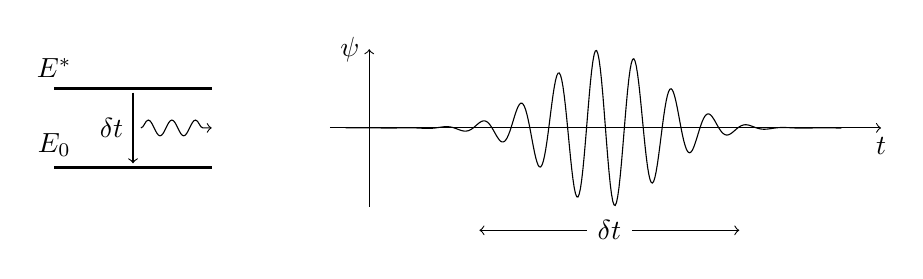
\begin{tikzpicture}
    \draw [->] (0,-1.) -- +(0,2) node [left]{$\psi$};
    \draw [->] (-0.5,0) -- +(7,0) node [below] {$t$};
    \draw [domain=-0.3:6, samples=400, variable=\t] 
      plot ({\t},{cos(\t*750)*exp(-(\t-3)^2)});
    \draw [<->] (1.4,-1.3) -- +(3.3,0) node[midway,fill=white,inner sep=4] {$\delta t$};
    \begin{scope}[xshift=-3cm]
      \draw [very thick] (-1,0.5) node[above] {$E^*$} -- (1,0.5);
      \draw [very thick] (-1,-0.5) node[above] {$E_0$} -- (1,-0.5);
      \draw [->] (0,0.45) -- (0,-0.45) node [midway, left]{$\delta t$};
      \draw [decorate,decoration={snake, amplitude=1mm,segment length=3mm,post length=1mm},->] (0.1,0) -- (1.,0);
    \end{scope}
  \end{tikzpicture}\par
  }
  \caption{Emissão de luz num processo de elementar (usou-se como exemplo aqui a
  emissão que acompanha uma transição atómica). Estes processos têm uma duração
  limitada. O pulso de ondas produzido tem uma duração
  semelhante. Só há correlação de fase dentro de cada pulso; logo, o tempo de
  coerência não pode exceder a sua duração.\label{fig:emission}}
\end{figure}
Paralelamente, outros pulsos são produzidos por outros processos que vão
ocorrendo na fonte de forma independente. Se as várias ondas produzidas deste
modo são independentes, elas não estão correlacionadas umas com as outras.
Assim, quaisquer correlações de fase podem apenas estabelecer-se dentro de
cada pulso de onda e por isso não podem manter-se ao longo de um intervalo de
tempo maior do que a própria duração do pulso. Assim, o tempo de coerência de
uma fonte luminosa tradicional (não laser) é, no máximo, igual à duração dos
pulsos gerados nos processos de emissão elementar que nela ocorrem.

Chama-se \emph{comprimento de coerência} à distância percorrida pela onda
durante o um intervalo de tempo igual ao tempo de coerência,
\begin{equation*}
l_c=c\tau_c,
\end{equation*}
onde $\tau_c$ é o tempo de coerência. Tendo em conta o parágrafo anterior,
deduzimos que o comprimento de coerência de um feixe de luz é o comprimento dos
pulsos de onda emitidos nos processos elementares de emissão que o geraram. O
significado físico do comprimento de coerência é semelhante ao do tempo de
coerência: a diferença de fases, num dado instante, de dois pontos dispostos
longitudinalmente no trajeto da onda tem um valor bem determinado ou muito
lentamente variável se a distância entre os pontos for inferior ao comprimento
de coerência; nessas condições a luz comporta-se como luz coerente. Se, ao
contrário,  distância entre os dois pontos considerados for maior que o
comprimento de coerência, então a diferença de fases é muito rapidamente
variável, ou seja, a luz comporta-se como incoerente.

\subsection{Coerência espacial. Raio de coerência}
Na secção anterior introduziu-se a coerência temporal de um feixe de luz e uma
noção com ela relacionada, a que pode dar-se o nome de \emph{coerência
longitudinal,} medida pelo valor do comprimento de coerência. Mas há ainda outro
parâmetro importante na descrição a coerência da luz. Há fenómenos de
interferência que envolvem pontos de uma mesma frente de onda, dispostos,
portanto, transversalmente à direção de propagação. A questão da coerência
nestes casos não se coloca em instantes diferentes nem (equivalentemente) em
pontos situados no trajeto da onda e, por isso, o tempo de coerência ou o
comprimento de coerência não servem para avaliar a correlação de fases que aqui
é relevante. 

Mas a situação é, em traços gerais, semelhante: se os dois pontos considerados
(recorde, estão situados transversalmente à direção de propagação) estiverem
suficientemente próximos um do outro, então a difereça de fases da onda nos dois
pontos é constante (se eles estiverem mesmo dispostos perpendicularmente à
propagação, até será nula) ou muito lentamente variável, mas essa constância
desaparece se eles se afastarem. O valor limiar da distância que separa estes
dois casos chama-se \emph{raio de coerência}.

Luz absolutamente coerente tem tempo de coerência, comprimento de coerência e
raio de coerência com valores infinitos. A luz das fontes tradicionais
(incoerente) tem comprimento e raio de coerência de apenas alguns nanómetros.
Entre estes dois extremos, a luz laser tem comprimentos de coerência muito
variados, que podem ir dos micrómetros (apontadores laser baratos) até às
dezenas de quilómetros.

Mais adiante neste capítulo, quando se discutirem fenómenos de interferência
concretos, será feita referência à coerência da luz envolvida e indicado qual o
parâmetro (comprimento de coerência ou raio de coerência) mais relevante em cada
caso.

\subsection{Interferência com radiação policromática}
Vimos já que só ocorre interferência\footnote{No sentido usual do termo, isto é,
com o estabelecimento de um padrão de interferência.} entre duas ondas
sinusoidais que se sobrepõem se elas tiverem a mesma frequência. Mas as ondas
verdadeiramente sinusoidais são uma idealização simplificadora, sem existência
real.  As ondas que encontramos no dia a dia e em laboratório não são
sinusoidais, mas podem ser descritas como a sobreposição de ondas sinusoidais
com diferentes frequências. Por exemplo, a luz do Sol é composta de diferentes
tipos de ondas eletromagnéticas sinusoidais, com frequências de toda a gama da
região visível do espectro (e mais infra-vermelho, rádio e um pouco de ultravioleta).

Uma onda não monocromática pode sempre ser escrita como uma soma de duas ou
mais ondas sinusoidais com diferentes frequências. Pode até ser necessário
considerar um número infinito, numerável ou não numerável, de componentes
sinusoidais.  Isto é, podemos escrever as duas ondas não sinusoidais que se
sobrepõem como
\begin{align*}
\Psi_1(\vec r,t)&=S_\omega\,\psi^{(1)}_\omega(\vec r,t)&
\Psi_2(\vec r,t)&=S_\omega\,\psi^{(2)}_\omega(\vec r,t),
\end{align*}
onde o símbolo $S_\omega f_\omega$ significa ``soma para todos os valores
relevantes de $\omega$ das quantidades $f_\omega$'' (esta soma pode ser um
somatório para valores discretos de $\omega$ e/ou um integral nos intervalos em
que $\omega$ varia continuamente) e $\psi_\omega(\vec r,t)$ representa uma
função sinusoidal com frequência $\omega$. Mas a onda resultante da sobreposição
destas duas ondas ondas num dado ponto e num dado instante é a \emph{adição} dos
valores que elas apresentam nesse ponto e nesse instante. Ora, a
adição é uma operação associativa, de forma que podemos escrever
\begin{align*}
\Psi(\vec r,t)&=\Psi_1(\vec r,t)+\Psi_2(\vec r,t)=
S_\omega\,\psi^{(1)}_\omega(\vec r,t)+
S_\omega\,\psi^{(2)}_\omega(\vec r,t)\\
&=S_\omega\,\left[\psi^{(1)}_\omega(\vec r,t)+
  \psi^{(2)}_\omega(\vec r,t)\right].
\end{align*}
Note-se que o termo entre parêntesis retos é o resultado da sobreposição das
componentes sinusoidais com frequência dada $\omega$ de cada uma das ondas;
ou seja, o resultado da sobreposição de duas ondas policromáticas pode
calcular-se somando os resultados da sobreposição das componentes de igual
frequência de cada onda.

Assim, na sobreposição de sinais policromáticos pode ocorrer interferência,
embora também possa não ocorrer (se os dois sinais não tiverem frequências em
comum, por exemplo). Como as condições de interferência construtiva ou
destrutiva dependem da frequência, os (eventuais) padrões de interferência da
sobreposição de feixes policromáticos costumam ter regiões distintas de
interferência construtiva ou destrutiva consoante a frequência. No caso da luz,
a diferentes frequências correspondem diferentes comprimentos de onda, logo,
diferentes cores. Assim, na interferência de luz policromática (por exemplo, de
luz branca) geram-se normalmente distribuições espaciais de cores diferentes.
Um exemplo destes padrões é ilustrado na Figura~\ref{fig:soapbubble}, que mostra
o reflexo da luz do céu numa bola de sabão.  A interferência que aqui ocorre (e
que estudaremos daqui a pouco) resulta da sobreposição dos reflexos na face
exterior e interior da película de água e sabão que forma a bolha.
\begin{figure}[htb]
{\centering
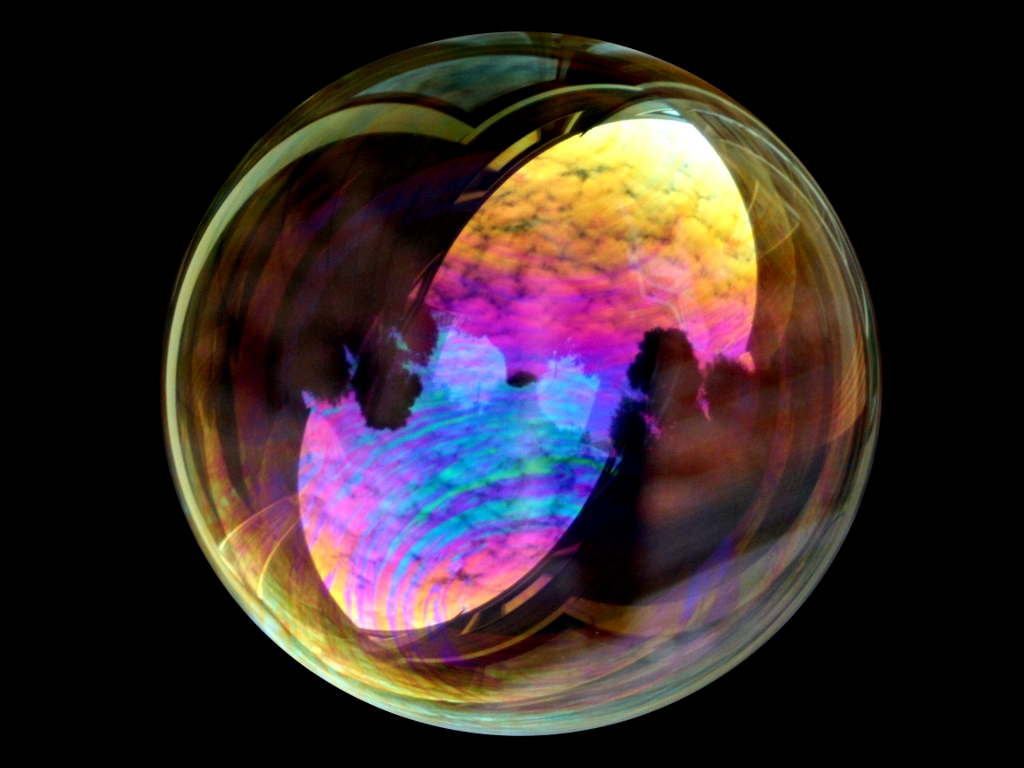
\includegraphics[width=0.3\linewidth]{figs/soap_bubble.jpg}\par
}
\caption{Padrão de cores resultante da interferência dos reflexos nas faces
exterior e interior da película de água que delimita uma bola de
sabão. (Retirado de
\protect\url{https://commons.wikimedia.org/wiki/File:Soap_bubble_sky.jpg}.)
\label{fig:soapbubble}}
\end{figure}


\section{Sobreposição de ondas eletromagnéticas}
Após esta interrupção no caminho que seguíamos para a discussão sobre a
coerência da secção anterior, retomemos o estudo da sobreposição de ondas,
considerando finalmente as que mais interessam na Ótica Física, as ondas de luz.
Nesta secção vamos essencialmente repetir o cálculo da
Secção~\ref{sec:scalarsuperp} com ondas de amplitude vetorial.

Consideremos então duas ondas eletromagnéticas planas sinusoidais com campo
elétrico $\vec E_1$ e $\vec E_2$, com as expressões características deste tipo
de onda,
\begin{align*}
\vec E_1=\vec E_1(\vec r,t)&=\vec A_1\cos(\vec k_1\cdot \vec r-\omega_1
t+\varphi_1)\\
\vec E_2=\vec E_2(\vec r,t)&=\vec A_2\cos(\vec k_2\cdot \vec r-\omega_2
t+\varphi_2).
\end{align*}
O campo elétrico resultante em cada ponto e instante é
\begin{equation*}
\vec E(\vec r, t)=\vec E_1(\vec r,t)+\vec E_2(\vec r,t).
\end{equation*}
Como vimos na Secção~\ref{sec:irradiance}, a irradiância de uma onda
eletromagnética é proporcional à média temporal do quadrado do campo elétrico,
tomada ao longo de um intervalo de tempo $\tau$ com a duração necessária para se
fazer a observação ou medição, muito mais longo do que o período das oscilações
das ondas de luz. Assim, representando a constante de proporcionalidade por
$\alpha$, podemos escrever
\begin{align}
I&=\alpha\langle E^2 \rangle_tau=
  \alpha\langle E_1^2 \rangle_\tau+
  \alpha\langle E_2^2 \rangle_\tau+
  2\alpha\langle \vec E_1\cdot\vec E_2 \rangle_\tau\nonumber\\
  &=I_1+I_2+I_{12},\label{eq:resirrad}
\end{align}
recuperando-se assim a eq.~\eqref{eq:superp2} que deduzimos na
Secção~\ref{sec:scalarsuperp}, mas com um termo de interferência que agora é
\begin{equation}
  I_{12}=2\alpha\langle \vec E_1\cdot\vec E_2\rangle_\tau.
\end{equation}
Ainda antes de continuar o cálculo podemos já establecer uma nova condição de
interferência para as ondas eletromagnéticas: não há interferência\footnote{No
sentido que demos a esta expressão: não se gera um padrão de interferência, com
regiões de reforço (interferência construtiva) e outras de atenuação
(interferência destrutiva) da intensidade luminosa.} se as duas ondas estiverem
polarizadas perpendicularmente, pois, nesse caso, $\vec E_1\cdot\vec E_2=0$ e o
termo de interferência anula-se.

A continuação do cálculo segue agora os mesmos passos que foram dados na
Secção~\ref{sec:scalarsuperp} para a sobreposição de ondas escalares.
Repetindo-os, obtemos\footnote{Omite-se o caso $\omega_1\neq\omega_2$ para aliviar a
notação; como para as ondas escalares, se as frequências são diferentes, o termo
de interferência anula-se.}
\begin{equation}
  I_{12}=\alpha \vec A_1\cdot\vec A_2\cos(\phi_1-\phi_2)=\alpha
  A_1A_2\cos\theta_{12}\cos(\phi_1-\phi_2),\qquad\text{ se }\omega_1=\omega_2,
\end{equation}
onde $\theta_{12}$ é o ângulo definido pelas direções de polarização das duas
ondas (é o ângulo entre $\vec E_1$ e $\vec E_2$). Tendo em conta as igualdades
da eq.~\eqref{eq:scalarwvint} (que foram deduzidas considerando ondas escalares
mas que, verifique-o, se mantêm com ondas electromagnéticas), o termo de
interferência pode ainda escrever-se numa forma em tudo semelhante à da
eq.~\eqref{eq:interft},
\begin{equation}\label{eq:interfvec}
  I_{12}=
  \begin{cases}
    2\sqrt{I_1I_2}\cos\theta_{12}\cos(\phi_1-\phi_2) & \text{ se
    }\omega_1=\omega_2\\
    0& \text{ se } \omega_1\neq\omega_2.
  \end{cases}
\end{equation}
Concluímos que as condições para a interferência de ondas de luz são semelhantes
às que establecemos para as ondas escalares, acrescentadas da condição de não
perpendicularidade das polarizações. Verificando-se interferência, ela é mais
perceptível se as polarizações das duas ondas tiverem a mesma orientação, uma ve
que é nessa situação que o produto escalar $\vec A_1\cdot\vec A_2$ (ou,
equivalentemente, o fator $\cos\theta_{12}$) tem o valor máximo. 

Ainda sobre a influência da polarização, note-se que dois raios de luz
não polarizados podem interferir, mesmo se não tem sentido, nesse caso, comparar
as orientações das suas polarizações. Mas passa-se aqui algo semelhante ao que
se referiu quando discutimos a interferência de radiação policromática, no final
da secção anterior: o resultado da sobreposição de dois raios de luz
despolarizados é a resultante das sobreposições das componentes de cada feixe
com igual polarização. Assim, quando se analiza a sobreposição de luz não
polarizada pode-se fazer a substituição $\cos\theta_{12}\rightarrow 0$. Pode
nestas condições ocorrer interferência (isto é, a
formação de um padrão de interferência), ou não, dependendo de outras
circunstâncias que não apenas a (des)polarização dos dois feixes.

Substituindo o resultado da eq.~\eqref{eq:interfvec} na eq.~\eqref{eq:resirrad},
resulta, para a irradiância da sobreposição,
\begin{equation}\label{eq:superp3}
  I=I_1+I_2+
  \begin{cases}
    2\sqrt{I_1I_2}\cos\theta_{12}\cos(\phi_1-\phi_2) & \text{ se
    }\omega_1=\omega_2\\
    0& \text{ se } \omega_1\neq\omega_2.
  \end{cases}
\end{equation}
Também agora notamos que, dados dois feixes de luz que se sobrepõem, a variável
determinante para a ocorrência numa dada região do espaço (e do tempo) de
interferência construtiva ou destrutiva é a diferença entre as suas fases em
cada ponto e instante dessa região.

%\textbf{Mudar isto. Irradiância proporcional ao valor médio do quadrado de E.}\\
%Consideremos duas ondas eletromagnéticas harmónicas planas numa região do
%espaço. Os campos elétrico e magnético da onda resultante são, de acordo com o
%princípio da sobreposição, as somas dos campos correspondentes de cada uma, isto
%é,
%\begin{align*}
%\vec E(\vec r,t)&=\vec E_1(\vec r,t)+\vec E_2(\vec r,t)&
%\vec B(\vec r,t)&=\vec B_1(\vec r,t)+\vec B_2(\vec r,t).
%\end{align*}
%A intensidade luminosa da onda resultante deve ser calculada como fizemos na
%Secção~\ref{sec:irradiance}, onde a definimos como a média temporal ao longo de
%um intervalo de tempo com duração razoável
%do módulo do vetor de Poynting, \begin{equation*}
%\vec S(\vec r,t)=\frac{1}{\mu_0}\vec E\times\vec B.
%\end{equation*}
%Dadas as expressões dos campos $\vec E$ e $\vec B$, o vetor de Poynting da
%sobreposição é
%\begin{align*}
%\vec S&=\frac{1}{\mu_0}(\vec E_1+\vec E_2)\times(\vec B_1+\vec B_2)=
%\frac{1}{\mu_0}\left(
%\vec E_1\times \vec B_1
%+\vec E_2\times \vec B_2
%+\vec E_1\times \vec B_2
%+\vec E_2\times \vec B_1
%\strut
%\right)\\
%&=\vec S_1+\vec S_2+\frac{1}{\mu_0}\left(
%\vec E_1\times \vec B_2
%+\vec E_2\times \vec B_1\right),
%\end{align*}
%onde $\vec S_1$ e $\vec S_2$ são os vetores de Poynting de cada onda.
%Mas nas ondas eletromagnéticas o campo magnético é determinado pelo campo
%elétrico (e vice versa); de acordo com a eq.~\eqref{eq:mf}, nas ondas planas
%temos
%\begin{equation*}
%\vec B = \frac{1}{\omega}\vec k\times\vec E=\frac{k}{\omega}\hat k\times\vec E=
%\frac{1}{c}\hat k\times\vec E,
%\end{equation*}
%onde $k=\|\vec k\|$ representa o módulo do vetor de onda e $\hat k=\vec k/k$ o
%versor (vetor unitário) com a orientação do vetor de onda. Substituindo acima,
%resulta
%\begin{equation*}
%\vec S=\vec S_1+\vec S_2+ \frac{1}{\mu_0c}\left[
%  \vec E_1\times\left(\hat k_2\times\vec E_2\right)
%  +\vec E_2\times\left(\hat k_1\times\vec E_1\right)
%  \right].
%\end{equation*}
%O produto vetorial triplo nestas expressões satisfaz as igualdades da
%eq.~\eqref{eq:tcp}, em particular,
%\begin{equation*}
%\vec a\times(\vec b\times\vec c)=\vec b\,(\vec a\cdot\vec c) - 
%\vec c\,(\vec a\cdot \vec b);
%\end{equation*}
%assim,
%\begin{align*}
%%\vec E_n\times\left(\hat k_n\times \vec E_n\right)&=
%%E_n^2\hat k_n-\vec E_n\,(\vec E_n\cdot\hat k_n)=E_n^2\,\hat k_n,\quad n=1,\,2\\
%\vec E_n\times\left(\hat k_m\times \vec E_m\right)&=
%(\vec E_n\cdot\vec E_m)\, \hat k_m-\vec E_m\,(\vec E_n\cdot\hat k_m),
%\quad n,\,m=1,\,2,\ m\neq n.
%\end{align*}
%O vetor de Poynting da sobreposição das duas ondas fica então com a forma
%\begin{equation*}
%\vec S=\vec S_1+\vec S_2 +\frac{1}{\mu_0c}\vec E_1\cdot\vec E_2(\hat k_1+\hat k_2)-
%\frac{1}{\mu_0c}
%  \left[\vec E_1\left(\vec E_2\cdot\hat k_1\right)+
%        \vec E_2\left(\vec E_1\cdot\hat k_2\right)\right]
%\end{equation*}
%
%Consideremos a situação particular (mas com muito interesse nas aplicações que
%estudaremos de seguida) em que as direções de propagação das duas ondas são
%praticamente iguais. Então os vetores $\vec S_1$, $\vec S_2$, $\hat k_1$ e $\hat
%k_2$ são quase paralelos; além disso o último termo no lado direito da equação
%acima pode desprezar-se porque, sendo comuns as direções de propagação das duas
%ondas, o campo elétrico de uma é também perpendicular ao vetor de onda da outra.
%Então, tem-se
%\begin{align*}
%\vec S&=\vec S_1+\vec S_2+\frac{2}{\mu_0c}\vec E_1\cdot\vec E_2\,\hat k,
%\end{align*}
%com $\hat k=\hat k_1=\hat k_2$. Uma vez que todos os vetores no lado direito têm
%a mesma direção (a da propagação de ambas as ondas), é trivial obter a expressão
%do módulo de $\vec S$,
%\begin{equation*}
%S=\|\vec S\|=S_1+S_2+\frac{2}{\mu_0c}\vec E_1\cdot\vec E_2.
%\end{equation*}
%Para obter a intensidade luminosa da sobreposição das duas ondas devemos agora
%calcular a média temporal desta expressão, resultando
%\begin{align}
%I&=\langle S_1\rangle+\langle S_2\rangle +
%  \frac{2}{\mu_0c}\left\langle\vec E_1\cdot\vec E_2\right\rangle\nonumber\\
%  &=I_1+I_2+ \frac{2}{\mu_0c}\left\langle\vec E_1\cdot\vec E_2\right\rangle,
%  \label{eq:interf}
%\end{align}
%onde a notação $\langle X\rangle$ representa a média temporal da função $X$.
%Esta igualdade mostra a intensidade luminosa da sobreposição de duas ondas não
%apenas soma das intensidades de cada uma, há ainda uma contribuição adicional,
%dita de \emph{interferência,} traduzida pelo terceiro termo no lado direito da
%eq.~\eqref{eq:interf}.
%
%Foquemo-nos no termo de interferência. A média temporal do produto escalar dos
%dois campos ao longo de um intervalo de tempo $0<t<\tau$ (que, recorde, deve ter
%uma duração $\tau$ muito maior do que operíodo da oscilação $T$) é
%\begin{equation*}
%\langle \vec E_1\cdot\vec E_2\rangle_\tau=\frac{1}{\tau}\int_0^\tau\vec
%E_1\cdot\vec E_2\,dt.
%\end{equation*}
%Os dois campos são, por hipótese, ondas planas, pelo que se podem escrever como
%\begin{align*}
%\vec E_1&=\vec A_1\cos(\Phi_1-\omega_1 t)&
%\vec E_2&=\vec A_2\cos(\Phi_2-\omega_2 t),
%\end{align*}
%ondese introduziram os símbolos $\Phi_i=\Phi_i(\vec r)=\vec k_i\cdot\vec r+\varphi_i,\
%i=1,\,2$. Então, substituindo em cima e desenvolvendo os cossenos usando
%fórmulas trignométricas elementares, temos
%\begin{align*}
%\langle\vec E_1\cdot\vec E_2\rangle_\tau&=\frac{1}{\tau}\vec A_1\cdot\vec A_2
%  \int_0^\tau\cos(\Phi_1-\omega_1 t)\cos(\Phi_2-\omega_2 t)\,dt\\
%  &=\frac{1}{\tau}\vec A_1\cdot\vec A_2\int
%    \left[\cos\Phi_1\cos\omega_1t+\sin\Phi_1\sin\omega_1t\right]
%    \left[\cos\Phi_2\cos\omega_2t+\sin\Phi_2\sin\omega_2t\right]\,dt\\
%  &=\vec A_1\cdot\vec A_2
%    \left[
%          \cos\Phi_1\cos\Phi_2\,\frac{1}{\tau}\int_0^\tau\cos\omega_1t\cos\omega_2t\,dt+\right.\\
%      &\hspace{2cm}
%         +\cos\Phi_1\sin\Phi_2\,\frac{1}{\tau}\int_0^\tau\cos\omega_1t\sin\omega_2t\,dt+\\
%      &\hspace{2cm}
%         +\sin\Phi_1\cos\Phi_2\,\frac{1}{\tau}\int_0^\tau\sin\omega_1t\cos\omega_2t\,dt+\\
%      &\hspace{2cm}+\left.
%          \sin\Phi_1\sin\Phi_2\,\frac{1}{\tau}\int_0^\tau\sin\omega_1t\sin\omega_2t\,dt
%    \right]
%\end{align*}
%

%%%%%%%%%%%%%%%%%%%%%%%%%%%%%%%%%%%%%%%%%%%%%%%%%%%%%%%%%%%%%%%%%%%%%%%%%%%%%%%%
\section{Experiência de Young}
A natureza ondulatória da luz foi demonstrada no final do séc.~XVIII por um
conjunto de observações, de que se destaca uma experiência de interferência da
luz que atravessa duas fendas paralelas, realizada por Young nos primeiros anos
do séc.~XIX.

Nesta experiência, faz-se incidir luz monocromática num alvo opaco com duas
aberturas com a forma de fendas finas, rectilíneas, paralelas e próximas uma da
outra, e observa-se a intensidade luminosa que é transmitida através das duas
fendas num ecrã colocado atrás do alvo (veja a Figura~\ref{fig:40-020}).
\begin{figure}[htb]
{\centering
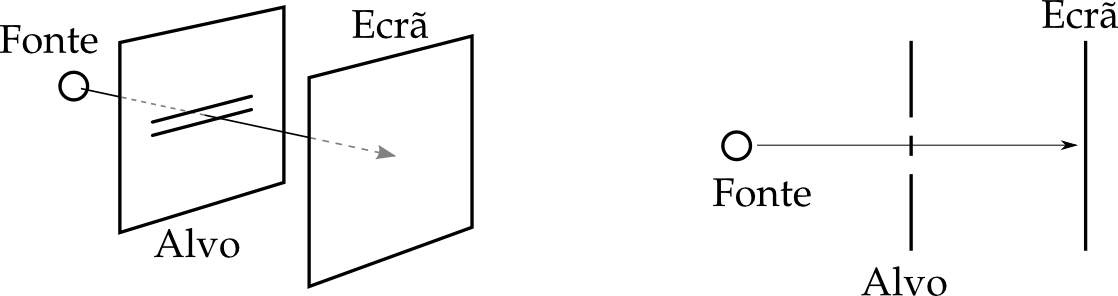
\includegraphics{figs/f40-020.png}
}\par
\caption{Experiência para demonstrar a interferência de dupla fenda de Young.
\label{fig:40-020}}
\end{figure}
Numa primeira abordagem, considerando apenas a lei da propagação retilínea da
luz, poderíamos pensar que o resultado desta experiência consiste na projeção
da sombra do alvo no ecrã, ficando nele definidas duas zonas iluminadas pela luz
que passa através de cada uma das fendas. No entanto, se as duas fendas
estiverem muito próximas uma da outra (a não mais do que uma ou duas décimas de
milímetro) vemos aparecer no ecrã uma série de faixas iluminadas paralelas,
como se tenta ilustrar na Figura~\ref{fig:40-030}.
\begin{figure}[htb]
    {\centering
        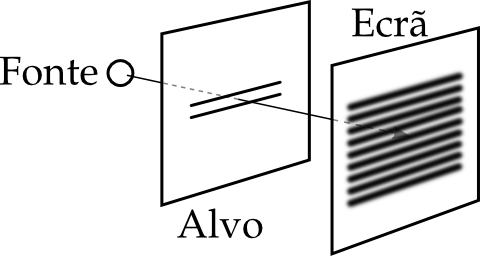
\includegraphics{figs/f40-030.png}
        \caption{Padrão de interferência característico de uma experiência de
            dupla fenda.\label{fig:40-030}}

    }
\end{figure}
Este resultado pode ser compreendido à luz do princípio de Huygens (ver a
Secção~\ref{sec:huygens}). A onda luminosa que se propaga para trás do alvo e que
atinge o ecrã é a sobreposição das duas ondas cilíndricas que têm origem em cada
uma das fendas. Nalgumas direções, essa sobreposição é construtiva, noutras é
destrutiva e daí resulta a sucessão de zonas iluminadas e obscuras no ecrã.
Tentemos analisar isto em mais detalhe.

Seja $\lambda$ o comprimento de onda da radiação usada, $a$ a distância entre
as duas fendas e $O$ um ponto situado sobre o alvo a igual distância ($a/2$, é
claro) de ambas. Seja $F$ a localização da fonte, considerada pontual. A direção
$FO$, que une a fonte ao ponto $O$ é a direção de incidência ou direção frontal.
Seja ainda $O'$ o ponto onde esta direção interseta o ecrã (veja a
Figura~\ref{fig:40-040}). Suponhamos que tanto a fonte de luz como o ecrã estão
muito afastados do alvo com as duas fendas, a distâncias muito maiores que
$\lambda$ ou $a$. As ondas originadas em cada fenda têm, aí, a mesma
fase (que é a da onda que nelas incidiu). Mas, até atingirem o ponto $P$,
percorrem distâncias diferentes. Logo, chegam a esse ponto com fases diferentes.
Calculemos esta diferença de fases. As distâncias percorridas pelas duas ondas,
que são as distâncias que separam cada fenda do ponto $P$, são dadas por
\begin{align*}
    s_1&=\sqrt{d^2+\left(y-\frac{a}{2}\right)^2}&
    s_2&=\sqrt{d^2+\left(y+\frac{a}{2}\right)^2}
\end{align*}
onde $d$ é a distância entre o alvo e o ecrã e $y$ é a distância $O'P$,
\begin{align*}
d&=\overline{OO'}&y&=\overline{O'P}.%&s&=\overline{OP}=\sqrt{d^2+y^2}.
\end{align*}
\begin{figure}[htb]
    {\centering
        \begin{tikzpicture}
\small
\coordinate(F) at (-3,0);
\draw [very thick] (F) circle(1mm) node[yshift=0.5cm]{$F$};
\draw [very thin, dotted] (0,0) -- (7,0);
\draw [line width=1mm] (0,-1) -- (0,-0.5) (0,-0.3) -- (0,0.3) (0,0.5) -- (0,2);
\draw [name path=s,line width=1mm] (6.5,-1) -- +(0,3);
\coordinate (O) at (0,0) node [left] {$O$};
\node at (6.5,0) [below right] {$O'$};

\path [name path=r] (0,0) -- (15:7);

\path [name intersections={of=r and s, by=P}];
\draw [dashed](O) -- (P) node [above left]{$P$};
\draw (15:2.5) arc (15:0:2.5) node [above right]{$\theta$};
\draw (0,-0.4) -- (P) node [pos=0.7, below]{$s_2$};
\draw (0,0.4) -- (P) node [pos=0.6, above]{$s_1$};

\draw [<->] (0.1,-0.9) -- (6.4,-0.9) node [midway,fill=white] {$d$};

\foreach \r in {0.7,0.9,1.1,1.3,1.5} {
\draw [gray] (F)+(-30:\r) arc (-30:30:\r);
}
\draw [->] (-2.2,0)--(-1.2,0);

\draw[<->] (7,0.1) coordinate(x) -- (x|-P) node [midway, fill=white]{$y$};
\draw [<->] (-0.75,-0.4) --(-0.75,0.4) node[midway,fill=white] {$a$};
\draw [thin, dotted] (0,-0.4) -- +(-0.9,0);
\draw [thin, dotted] (0,0.4) -- +(-0.9,0);
\end{tikzpicture}

        \caption{Geometria da experiência de Young para demonstrar a
        interferência de dupla fenda.\label{fig:40-040}}

    }
\end{figure}
Como a distância entre as fendas é muito menor do que a distância alvo-ecrã,
são válidas as aproximações\footnote{Estas expressões foram obtidas usando a
fórmula de Taylor até à primeira ordem. Com uma calculadora, faça uma estimativa
do erro das aproximações para $d=1$\,m; $a=0,1$\,mm, $y=1$\,cm.}
\begin{align*}
s_1\simeq s-\frac{y}{s}\frac{a}{2}\\
s_2\simeq s+\frac{y}{s}\frac{a}{2},
\end{align*}
onde $s=\overline{OP}=\sqrt{d^2+y^2}$ representa a distância entre o ponto $O$ e
o ponto $P$.

Seja $\varphi_0$ a fase inicial (comum, já o constatámos) das duas ondas. As
fases com que atingem o ponto $P$, de acordo com a eq.~\eqref{eq:deltaphix}, são
então dadas por 
%fórmula deduzida na Secção~\ref{sec:dfidx}, são então dadas por
\begin{align*}
\varphi_1 &= \varphi_0+2\pi\frac{s_1}{\lambda}&
\varphi_2 &= \varphi_0+2\pi\frac{s_2}{\lambda};
\end{align*}
logo, a diferença de fase com que atingem o ponto $P$ resulta
\begin{equation}\label{eq:youngdf1}
\delta\varphi = \varphi_2-\varphi_1 =2\pi\frac{s_2-s_1}{\lambda}=
2\pi\frac{a}{\lambda}\,\frac{y}{s},
\end{equation}
ou, como função de $\sin\theta=y/s$,
\begin{equation}\label{eq:youngdf2}
\delta\varphi = 2\pi\frac{a}{\lambda}\sin\theta.
\end{equation}

Agora que temos uma expressão para a diferença de fase das duas ondas que
atingem um ponto arbitrário no ecrã, podemos aplicar as condições que
estabelecemos na Secção~\ref{sec:condint} e ver em que direções ocorre
interferência construtiva (reforço da irradiância) ou destrutiva (atenuação da
radiância)
%usar a fórmula deduzida na
%Secção~\ref{sec:sobrpos} para calcular a amplitude da onda resultante. Mas neste
%momento é mais interessante perceber em que direções ocorre interferência
%construtiva (direções em que aquela amplitude tem um valor elevado) ou
%destrutiva (aquelas onde a amplitude se anula). Para isso, chega 
Temos então o seguinte
\begin{itemize}
\item
    \textbf{Direções em que ocorre interferência construtiva}\\
    São aquelas para as quais se verifica
    \begin{align*}
    \delta\varphi &= 2\pi\frac{a}{\lambda}\sin\theta=
                    2l\pi,\quad\text{com }l=0,\pm1,\pm2,\ldots
    \end{align*}
    ou seja, aquelas que fazem com a direção de incidência um ângulo $\theta$
    dado por
    \begin{equation}\label{eq:youngc}
      \sin\theta=l\;\frac\lambda a,\quad l=0,\pm1,\pm2,\ldots
    \end{equation}
\item
    \textbf{Direções em que ocorre interferência destrutiva}\\
    Nestas direções a diferença de fase deve ser um múltiplo semi-inteiro de
    $2\pi$, isto é,
    \begin{equation*}
        \delta\varphi=2\pi\frac{a}{\lambda}\sin\theta=2\left(l\pm\frac12\right)
        \pi,\quad k=0,\pm1,\pm2,\ldots
    \end{equation*}
    de onde resulta
    \begin{equation}\label{eq:youngd}
        \sin\theta=\left(l\pm\frac12\right)\frac\lambda a,\quad
        l=0,\pm1,\pm2,\ldots
    \end{equation}
\end{itemize}
Claro que, nas eqs.~\eqref{eq:youngc} e~\eqref{eq:youngd}, não faz sentido dar
ao inteiro $l$ valores tais que resultem para $\sin\theta$ valores maiores
do que 1. Por isso, o número de máximos (logo, de mínimos) de interferência numa
experiência de Young fica condicionado pelo valor de $a/\lambda$. Mais
concretamente, o número de máximos é dado por
\begin{equation*}
  N_\text{mx}=2\,\text{int}(\frac{a}{\lambda}) + 1,
\end{equation*}
onde $\text{int}(x)$ representa a parte inteira de $x$.



A intensidade luminosa incidente no ecrã pode calcular-se substituindo a
expressão da diferença de fase da eq.~\eqref{eq:youngdf1} na
eq.~\eqref{eq:superp3}. Pela simetria da exposição das duas fendas, devemos
tomar iguais as irradiâncias das duas ondas, $I_1=I_2=I_f$ ($I_f$ representa
aqui a irradiância da luz que atravessa cada fenda); além disso, as frequências
das duas ondas que se sobrepõem são iguais à frequência da luz usada na
experiência, $\omega_1=\omega_2=\omega$; por fim, as ondas que atravessam as
duas fendas têm também a mesma polarização (ou são ambas despolarizadas), igual
à da luz incidente no alvo com as fendas. Assim, nesta situação a
eq.~\eqref{eq:superp3} toma a forma
\begin{align*}
I&=2I_f+2I_f\cos\delta\varphi=
  2I_f(1+\cos\delta\varphi)\\&=4I_f\cos^2\frac{\delta\varphi}{2},
\end{align*}
tendo-se usado a igualdade trignométrica $\cos\alpha=2\cos^2(\alpha/2)$. Com
$\delta\varphi$ dado pela eq.~\eqref{eq:youngdf2}, obtemos
\begin{equation}\label{eq:yngi}
I=4I_f\cos^2\left(\pi\frac{a}{\lambda}\sin\theta\right).
\end{equation}
O gráfico desta função está ilustrado na Figura~\ref{fig:yngint}. Notam-se
oscilações regulares entre valores máximos ($4I_f$) e mínimos (0), que ocorrem
nas direções previstas nas eqs.~\eqref{eq:youngc} e~\eqref{eq:youngd},
respetivmente.
\begin{figure}[htb]
  {\centering
  \begin{tikzpicture}[]
    \small
    \pgfmathsetmacro{\s}{1.75}
    \draw [->] (-3.1,0)--(3.1,0) node [below] {$\theta$};
    \draw [->] (0,-0.05) node [below] {0}-- (0,2) node [right]{$I$};
    \draw [samples=200, domain=-1.55:1.55, thick, variable=\q]
      plot ({\s*\q},{1.5*
              (cos(deg(pi*2.5*sin(deg(\q)))))^2});
    \draw (\s*pi/2,0.05) -- +(0,-0.1) node [below] {$\frac\pi2$};
    \draw (-\s*pi/2,0.05) -- +(0,-0.1) node [below] {$-\frac\pi2$};
    \node at (0,1.5) [above left]{$4I_f$};
    \node at (7,0.8) {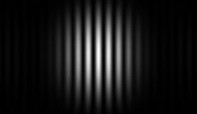
\includegraphics[height=2.6cm]{figs/twoslitinterf.jpg}};
  \end{tikzpicture}\par}
  \caption{\label{fig:yngint}Gráfico da intensidade da interferência de Young
    com $a/\lambda=2,5$ (à esquerda) e fotografia do ecrã iluminado numa
    experiência concreta. (Desconheço os parâmetros desta experiência, a figura
    foi adaptada de \protect\url{http://www.okotech.com/lp-interference}.)}
\end{figure}
A estas direções
correspondem, no ecrã, faixas alternadamente iluminadas e escurecidas,
muito aproximadamente equidistantes umas das outras. Para o verificar, note que
$\sin\theta=y/d$ (reveja a Figura~\ref{fig:40-040}) e que, para pequenos
ângulos, $s\simeq d$. Assim,
\begin{equation*}
  I=4If\cos^2\left(\pi\frac{a}{\lambda}\sin\theta\right)\simeq
  4I_f\cos^2\left(\pi\frac{a}{\lambda}\frac{y}{d}\right).
\end{equation*}
À medida que $y$ aumenta a partir da posição central $y=0$, esta função oscila
repetidamente entre os valores mínimo (0) e máximo ($4I_f$), encontrando-se os
máximos sucessivos afastados de $2\lambda d/a$.  A Figura~\ref{fig:yngint}
apresenta também, no lado direito, este padrão de máximos e mínimos
equidistantes, fotografado numa experiência concreta de interferência de fenda
dupla.

\section{Redes de difração 1} 
As redes de difração são dispositivos óticos interferométricos com muitas
aplicações. As mais simples, que estudaremos agora, consistem num meio
transparente no qual está gravada uma sucessão de riscos retilíneos, paralelos
e opacos muito próximos (não mais do que poucas décimas de milímetro), entre os
quais a luz pode passar\footnote{Redes como as que acabei de descrever são as
  mais simples e vulgares. Outros tipos de rede podem ter riscos circulares
  concêntricos, riscos retilíneos que divergem de um ponto, arranjos regulares
  de pequenas ``janelas'' num fundo opaco, etc.}. Quando um feixe de luz incide
numa rede de difração, as frentes de onda fragmentam-se, dividindo-se pelas
faixas transparentes entre os riscos, e na luz transmitida ocorre interferência
entre as diferentes ondas resultantes daquela fragmentação.  Assim, uma destas
rede de difração é um pouco como as fendas duplas da interferência de Young, à
parte o facto de serem muitas fendas e não apenas duas. 

O padrão de interferência produzido por uma rede de difração tem um aspeto em
comum com o da interferência de fenda dupla: as direções em que ocorre
interferência construtiva (aquelas onde se dá um reforço da intensidade
luminosa) satisfazem uma relação em tudo idêntica à da
eq.~\eqref{eq:youngc}, que deduzimos na secção anterior (o parâmetro $a$
até mantém, ainda, o significado que já tinha, da distância entre as faixas por
onde a luz passa). Mas as semelhanças acabam aí. Enquanto que a intensidade da
interferência na experiência de Young é a função oscilante, mas contínua e
regular, da direção apresentada no gráfico da Figura~\ref{fig:yngint}, a da
interferência numa rede de difração, sobretudo se tiver muitos riscos por
unidade de comprimento, é descontínua; é nula em todas as direções, excepto
naquelas em que ocorre interferência totalmente construtiva. O gráfico da
Figura~\ref{fig:gratingi} ilustra a diferença entre as duas situações.
\begin{figure}[htb]
{\centering
  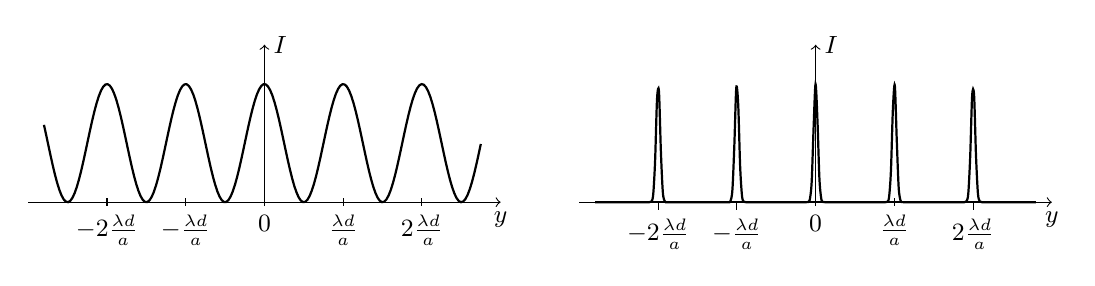
\begin{tikzpicture}[]
    \small
    \draw [->] (-3,0)--(3,0) node [below] {$y$};
    \draw [->] (0,-0.05) node [below] {0}-- (0,2) node [right]{$I$};
    \draw [samples=200, domain=-2.8:2.75, thick, variable=\y]
      plot ({\y},{1.5*(cos(\y*180))^2});
    \draw (1,0.05) -- +(0,-0.1) node [below] {$\frac{\lambda d}{a}$};
    \draw (2,0.05) -- +(0,-0.1) node [below] {$2\frac{\lambda d}{a}$};
    \draw (-1,0.05) -- +(0,-0.1) node [below] {$-\frac{\lambda d}{a}$};
    \draw (-2,0.05) -- +(0,-0.1) node [below] {$-2\frac{\lambda d}{a}$};
    %\node at (0,1.5) [left]{$4I_f$};
	  \begin{scope}[xshift=7cm]
      \draw [->] (-3,0)--(3,0) node [below] {$y$};
      \draw [->] (0,-0.05) node [below] {0}-- (0,2) node [right]{$I$};
      \draw [thick] (-2.8,0) -- (2.8,0);

      \draw (1,0.05) -- +(0,-0.1) node [below] {$\frac{\lambda d}{a}$};
      \draw (2,0.00) -- +(0,-0.1) node [below] {$2\frac{\lambda d}{a}$};
      \draw (-1,0.00) -- +(0,-0.1) node [below] {$-\frac{\lambda d}{a}$};
      \draw (-2,0.00) -- +(0,-0.1) node [below] {$-2\frac{\lambda d}{a}$};
      \draw [samples=229, smooth, domain=-2.8:2.8, thick, variable=\y]
        plot ({\y},{1.5*(exp(-700*(\y+2)^2)+
                         exp(-700*(\y+1)^2)+
                         exp(-700*(\y+0)^2)+
                         exp(-700*(\y-2)^2)+
                         exp(-700*(\y-1)^2))
        });
    \end{scope}
  \end{tikzpicture}\par
}
\caption{\label{fig:gratingi}Intensidade da interferência numa fenda dupla de
Young (à esquerda) e numa rede de difração (à direita). Quanto mais próximos
forem os riscos na rede de difração, mais estreitos são os picos de
interferência representados no gráfico da direita. Para $a\simeq 10\,\mu$m
(ordem de grandeza bastante típica), estes picos teêm espessura imperceptível.
Ou seja, nesses casos as redes de difração só transmitem luz com um dado
comprimento de onda nalgumas direções bem determinadas.}
\end{figure}


Tentemos perceber a interferência numa rede de difração, fazendo o cálculo da
intensidade da sobreposição das ondas que atravessam cada fenda.
 Nesta análise usaremos ondas escalares como as da
Secção~\ref{sec:scalarsuperp} porque as considerações sobre a polarização são,
aqui, irrelevantes (como já o foram na análise da experiência de
Young).

Consideremos um feixe paralelo de luz monocromática com comprimento de onda que
$\lambda$ incide perpendicularmente numa rede de difração com fendas separadas
por uma distância $a$. São iluminadas um número $N$ destas fendas, que
numeramos sequencialmente de 1 a $N$ (veja a Figura~\ref{fig:gratingb}). A luz
transmitida pela rede vai incidir num ecrã situado a uma distância $d$, onde se
forma e é observado o padrão de interferência.
\begin{figure}[htb]
  {\centering
    \begin{tikzpicture}
      \small\sffamily
      \pgfmathsetmacro{\q}{9}
      \pgfmathsetmacro{\l}{7}
      \draw [thin, ->] (0,0) -- (0,1.2) node [right]{$y$};
      \node at (0,-0.5) [below, scale=0.8]{RD};
      \draw [thin,->](-0.25,0) -- ({1.1*\l},0) node[below] {$x$};
      \draw [dashed] (0,0) coordinate(O) -- (\q:\l) coordinate(p) node [above
        left]{$P$};

      \foreach \y [remember=\y as \oldy (initially -0.6), count=\i] in
        {-0.25, 0.2, 0.65} {
          \draw [->-] (0,\y) node [xshift=-2mm, scale=0.7] {\i}-- (p);
          \draw [ultra thick] (0,\oldy+0.05) -- (0,\y-0.05);
        }
      \draw [ultra thick] (0,0.7) -- (0,1);
      \draw (1.75,0) arc (0:\q:1.75) node
        [circle,shift={(3mm,-1.5mm)}, fill=white, inner sep=0] {$\theta$};
      \coordinate (s) at (p|-O);
      \draw [thick] ($ (p)!-2mm!(s) $) -- ($ (s)!-5mm!(p) $) node
          [below, scale=0.8]{E};
      \foreach \y in {-0.35, 0.05, 0.45, 0.85} {
        \draw [thin,->] (-0.8,\y) --+(0.3,0);
      }
      \draw [<->]([shift={(2mm,0.3mm)}]s) -- ([shift={(2mm,-0.3mm)}]p)
        node [midway, right]{$y$};
      \draw [<->] (0.1,-0.4) -- ([xshift=-2mm]\l,-0.4)
        node [midway, fill=white, inner sep=1] {$d$};
    \end{tikzpicture}\par
  }
  \caption{\label{fig:gratingb}Rede de difração exposta a um feixe paralelo de
    luz monocromática (neste diagrama, apenas são expostas três faixas de
  transmissão da rede).}
\end{figure}
Consideraremos no que se segue que a distância rede de difração--ecrã é muito
maior que o comprimento de onda da luz, que a distância entre as fendas da rede
de difração e que a zona iluminada da rede, isto é,
\begin{align*}
  d&>>\lambda,&d&>>a, & d&>>Na.
\end{align*}
Com esta suposição simplificamos bastante os cálculos porque podemos tratar as
ondas que atingem o ecrã provenientes de cada fenda na rede de difração como
ondas planas com igual amplitude. Em contrapartida, devemos ter presente que os
resultados que vamos obter não se verificam em pontos próximos da rede de
difração, onde a suposição deixa de ser válida.

Tomemos um sistema de coordenadas cartesiano, com origem num ponto da rede de
difração mais ou menos próximo do centro da zona iluminada (não é muito
importante), com o eixo dos $x$ paralelo à direção de incidência e com o dos $y$
perpendicular a essa direção e também à dos riscos da rede. Assim, os pontos da
rede têm coordenada $x$ nula e os do ecrã têm-na igual a $d$. Seja $y_l$ ($l=1,\
2,\ \ldots,\ N$) a coordenada $y$ da $l$-ésima fenda exposta da rede de
difração.  Como se encontram igualmente espaçadas de uma distância $a$, temos
\begin{equation}\label{eq:ydist}
  y_l = y_0+la,
\end{equation}
onde $y_0$ é uma constante arbitrária relacionada com a posição do ponto que
escolhemos como origem\footnote{$y_0$ é apenas a coordenada $y$ de um ponto
  situado uma distância $a$ abaixo da fenda número 1.}. A distância que separa
um ponto $P$ arbitrário do ecrã com coordenadas $(d,y)$ da $l$-ésima fenda da
rede de difração é
\begin{equation*}
  s_l=\sqrt{d^2+(y-y_l)^2}=\sqrt{d^2 + y^2 - 2yy_l+y_l^2}.
\end{equation*}
Mas a soma de quadrados $d^2+y^2$ é igual ao quadrado da distância da origem ao
ponto do ecrã considerado, que representaremos por $s$. Por outro lado, estando o
ecrã muito afastado da rede de difração, esta distância $s$ é muito maior que as
distâncias entre as várias fendas iluminadas; assim, podemos desprezar $y_l^2$
face a $s^2$, e resulta então
\begin{equation}\label{eq:grdist}
  s_l=\sqrt{s^2-2yy_l}=s\sqrt{1-2\frac{yy_l}{s^2}}\simeq
  s-\frac{yy_l}{s}=s-y_l\sin\theta,
\end{equation}
onde se usou a aproximação $\sqrt{1+x}\simeq1+x/2$, válida para $x<<1$, e se
introduziu o ângulo $\theta$ entre a direção de incidência e a do
vetor posição do ponto $P$.

A luz que atravessa a rede de difração através da fenda número $l$ tem no ponto
$P$ função de onda que, usando a notação complexa e o resultado da
eq.~\eqref{eq:grdist}, se pode escrever como
\begin{equation*}
  \psi_l(P,t) = Ae^{i(ks_l-\omega t)}=Ae^{i(ks-\omega t)}
  e^{iky_l\sin\theta},
\end{equation*}
onde $k=2\pi/\lambda$, $A$ é uma constante que representa a amplitude desta
onda e se descartou uma constante de fase aqui irrelevante (podemos fazê-lo
porque supomos que a luz que incide na rede de difração tem uma fase comum e,
por isso, que a fase inicial das várias ondas transmitidas é igual). De acordo
com o princípio da sobreposição, o sinal ondulatório no ponto $P$ do ecrã é a
soma das várias contribuições,
\begin{equation}\label{eq:grtsuperp}
  \psi(P)=\sum_{l=1}^N\psi_l(P) =
    Ae^{i(ks-\omega t)} \sum_{l=1}^Ne^{iky_l\sin\theta}=
    Ae^{i(ks-\omega t+ky_0\sin\theta)}\sum_{l=1}^Ne^{ikla\sin\theta},
\end{equation}
tendo-se substituido aqui a expressão da eq.~\eqref{eq:ydist}. 

Foquemos a atenção no somatório no lado direito desta igualdade. Com
$u=ka\sin\theta$ para aligeirar a notação, este somatório pode escrever-se como
\begin{equation*}
  \sum_{l=1}^Ne^{iul} = \sum_{l=1}^N\left(e^{iu}\right)^l,
\end{equation*}
ou seja, é a soma dos $N$ primeiros termos termos de uma sucessão geométrica de
razão $e^{iu}$\footnote{Uma sucessão geométrica com razão $r$ é
  uma sucessão cujo termo geral é da forma $v_l=r^l$; a soma dos primeiros
  termos é dada por
  \begin{equation*}
    \sum_{l=1}^Nr^l=r\frac{1-r^N}{1-r}.
  \end{equation*}
}, dada por
\begin{align*}
  \sum_{l=1}^N\left(e^{iu}\right)^l&=
    e^{iu}\frac{1-e^{iNu}}{1-\e^{iu}}=
    e^{iu}\frac{e^{iuN/2}}{e^{iu/2}}
    \frac{e^{-iuN/2} - e^{iuN/2}}{e^{-iu/2}-e^{iu/2}}
\end{align*}
Mas $e^{ix}-e^{-ix}=2i\sin x$, de forma que este somatório fica
\begin{equation*}
  \sum_{l=1}^N\left(e^{iu}\right)^l=
    e^{iu(N+1)/2}\;\frac{\sin(Nu/2)}{\sin(u/2)}. 
\end{equation*}
Substituindo na eq.~\eqref{eq:grtsuperp} obtemos a expressão para o cálculo da
função de onda no ponto $P$:
\begin{equation}\label{eq:grtwav}
  \psi(P,t)=A\frac{\sin(Nu/2)}{\sin(u/2)} 
    e^{i\left(ks-\omega t+\varphi(\theta)\right)},
\end{equation}
onde $\varphi(\theta)$ é uma constante de fase que depende da direção $\theta$,
dada por
\begin{equation*}
  \varphi(\theta)=k\left(\frac{N+1}{2}a+y_0\right)\sin\theta,
\end{equation*}
que até pode ser tomada igual a zero, escolhendo a origem do sistema de
coordenadas de tal forma que $y_0=-(N+1)a/2$, ou seja, escolhendo-a no centro
da zona iluminada.

A expressão da eq.~\eqref{eq:grtwav} representa uma onda monocromática com
amplitude
\begin{equation}
  A_r=A\frac{\sin(Nu/2)}{\sin(u/2)}.
\end{equation}
A intensidade luminosa no ponto $P$ é, como sempre, proporcional ao quadrado da
amplitude. Assim, resulta por fim
\begin{equation}\label{eq:gratint}
  I(P) = I_f\left(\frac{\sin(Nu/2)}{\sin(u/2)}\right)^2,\qquad\text{com }
  u=ka\sin\theta=2\pi\frac{a}{\lambda}\sin\theta,
\end{equation}
onde $I_f$ é a intensidade, no ponto $P$, das ondas que passam através de cada
fenda da rede de difração.

Fazendo $N=2$ na equação eq.~\eqref{eq:gratint} recuperamos, como seria de
esperar, a fórmula que deduzimos para a experiência de Young, da
eq.~\eqref{eq:yngi}\footnote{Fica como exercício fazer esta dedução.
  Sugestão: note que $\sin x=2\sin(x/2)\cos(x/2)$.}. A Figura~\ref{fig:gratint2}
ilustra o gráfico da intensidade transmitida por uma rede de difração (com
$a/\lambda=2,5$) como função de $\theta$ para diferentes valores de $N$.
\begin{figure}[htb]
  {\centering
    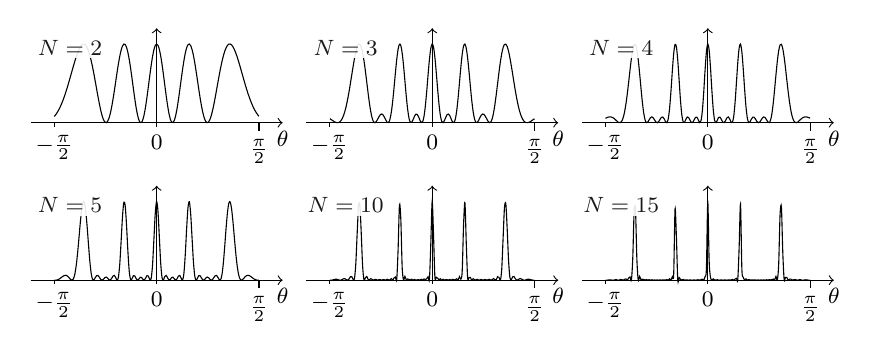
\begin{tikzpicture}
      \footnotesize
      \foreach \n [count=\i from 0] in {2,3,4,5,10,15} {
        \pgfmathsetmacro{\x}{int(Mod(\i,3))}
        \pgfmathsetmacro{\y}{int(\i/3)}
        \pgfmathsetmacro{\al}{pi*2.5}
        \begin{scope}[shift={(\x*3.5,-\y*2)}]
          \draw [thin, ->] (-1.6,0) -- (1.6,0) node [below]{$\theta$};
          \draw (1.3,0)--+(0,-0.1) node [below]{$\frac{\pi}{2}$};
          \draw (-1.3,0)--+(0,-0.05) node [below]{$-\frac{\pi}{2}$};
          \draw [thin, ->] (0,-0.05) node[below]{0} -- (0,1.2);
          \draw [thin, domain=-1.3:1.3, variable=\x,smooth, samples=151]
            plot (\x,
             {(sin(deg(\n*\al*sin(deg(\x))))/sin(deg(\al*sin(deg(\x))))/\n)^2});
          \node [fill=white, fill opacity=0.90, inner sep=1] at (-1.1,0.95)
             {$N=\n$};
        \end{scope}
      }
    \end{tikzpicture}
    \par
  }
  \caption{\label{fig:gratint2}Intensidade da transmissão por uma rede de
    difração com $a/\lambda=5/2$ como função do ângulo com a direção de
    incidência, para diferentes valores do número de fendas da rede que
    participam no processo interferométrico. Os máximos ocorrem para
    $\sin\theta=l\lambda/a$, $l=0,\ \pm1,\ \pm2, \ldots$, independentemente de
    $N$. Mas para $N$ grande, a intensidade transmitida é nula em práticamente
    todas as direções, à exceção daquelas que que se verificam os máximos.}
\end{figure}
Para $N=2$ resulta a oscilação regular já antes calculada para a experiência de
Young (reveja a Figura~\ref{fig:yngint}). Mas nota-se que à medida que aumenta
$N$ os máximos se vão tornando cada vez mais estreitos e a intensidade
resultante entre os máximos vai ficando cada vez menor, como se ilustrou na
Figura~\ref{fig:gratingi}.



\section{Interferência em reflexões múltiplas}
\begin{wrapfigure}[10]{l}{0.3\textwidth}
    {\centering
        \usetikzlibrary{decorations.markings,intersections}
\tikzset{->-/.style={decoration={
  markings,
  mark=at position .5 with {\arrow{>}}},postaction={decorate}}}
\tikzset{-<-/.style={decoration={
  markings,
  mark=at position .5 with {\arrow{<}}},postaction={decorate}}}
\begin{tikzpicture}
\fill [gray!10](-0.8,-1.) rectangle(0.8,1.25);
\draw [name path=s2, thick] (0.8,-1.) -- +(0,2.25);
\draw [name path=s1, thick] (-0.8,-1.) -- +(0,2.25);
\node at (-1.2,1.1) {$n_1$};
\node at (0.1,1.1) {$n_2$};
\node at (1.2,1.1) {$n_3$};

\coordinate(p1) at (-0.8,0.5);
\draw [-<-](p1) --+(155:1.5) node[below] {$r_0$};
\draw [->-](p1) --+(205:1.5) node[above]{$r_1$};
\path[name path=r](p1)--+(-7:2.2);
\path[name intersections={of=s2 and r, by=p2}];
\draw [->-] (p1)--(p2) node [pos=0.3,above] {$r'_1$};
\draw [->,dashed] (p2)--+(-30:0.8);

\path [name path=r](p2) --+(187:2.2);
\path[name intersections={of=s1 and r, by=p3}];
\draw [->-](p2)--(p3) node[pos=0.3,below]{$r'_2$};
\draw [->-] (p3) -- +(205:1.5) node[below]{$r_2$};
\draw [->,dashed] (p3)--+(-7:0.6);
\end{tikzpicture}
        \caption{Interferência em reflexões múltiplas.\label{fig:40-050}}

    }
\end{wrapfigure}
Considere uma película fina de um meio transparente, como a que constitui a
superfície de uma bola de sabão, a camada oleosa que frequentemente se nota nos
charcos de água em parques de estacionamento ou a cobertura anti-reflexos de
algumas lentes oftálmicas. Quando a luz incide numa destas películas, uma parte
é refletida na face onde se dá a incidência, mas outra parte é refratada para o
interior, atravessando a película até atingir a face oposta. Aí, ocorre um novo
processo de separação: uma parte é refratada para o exterior da película, a
outra é refletida de volta para a face onde se deu a incidência. Uma parte deste
raio é refratado, sobrepondo-se ao raio que se refletiu logo no momento da
primeira incidência. Como estes dois raios (o que se refletiu na face de
incidência inicial e o que se refletiu na face oposta) percorrem trajetos
diferentes e sofrem processos diferentes, apresentam, em geral, fases diferentes
quando interferem. Em que condições é essa interferência construtiva ou
destrutiva?

A resposta genérica a esta pergunta é a do costume, estabelecida na
Secção~\ref{sec:condint}: se a diferença entre as fases dos dois raios
refletidos ($r_1$ e $r_2$ na Figura~\ref{fig:40-050}) for um múltiplo inteiro de
$2\pi$, a interferência é construtiva e o reflexo, consequentemente, intenso; ao
contrário, se essa diferença de fase for um múltiplo semi-inteiro de $2\pi$, a
interferência é destrutiva, logo, o reflexo é atenuado. Devemos agora encontrar
uma expressão para a diferença de fase entre os dois raios neste problema, para
podermos concretizar esta solução. Para isso, devemos analisar os vários
processos por que passam os dois raios.

O raio que se reflete na superfície de incidência (identificado como $r_1$ na
Figura~\ref{fig:40-050}) sofre apenas o próprio processo de reflexão; o raio que
se reflete na face oposta ($r_2$), para além da reflexão, passa ainda por duas
refrações (à entrada e à saída da película) e propaga-se dentro da película
percorrendo a sua espessura nos dois sentidos. Cada um destes processos tem que
ser analisado separadamente.

\subsection*{Alterações de fase na reflexão}
As reflexões (como as refrações) são processos temporalmente descontínuos e,
por isso, é crível que possam ser acompanhadas de alterações descontínuas também
das propriedades das ondas de luz que os sofrem, incluindo da sua fase. De
facto, nas reflexões podem ocorrer (mas não ocorrem sempre) variações de fase.
Mais concretamente, verifica-se o seguinte:
\begin{itemize}
\item
    quando o índice de refração do meio onde se propaga a luz incidente é
    \emph{menor} do que o do meio contra o qual se faz a incidência, então
    \emph{ocorre uma inversão de fase}, ou seja, o raio refletido tem uma fase
    adiantada (ou atrasada, vai dar no mesmo) de $\pi$ relativamente à do raio
    incidente.
\item
    quando o meio onde se propaga a luz incidente tem índice de refração
    \emph{maior} do que o do meio contra o qual a luz incide, \emph{não há}
    qualquer variação de fase, ou seja, o raio refletido tem a mesma fase que o
    raio incidente;
\end{itemize}

Este fenómeno é semelhante à variação de fase sofrida pela reflexão de uma onda
mecânica numa corda esticada num ponto da corda onde se unem zonas de densidade
diferente. Neste caso, constata-se que se a onda se propaga numa zona da corda
de densidade mais baixa, a onda refletida tem a fase invertida relativamente à
onda incidente; mas se a onda incidente se propaga na zona da corda de densidade
mais elevada, então a onda refletida tem fase idêntica à da incidente (veja a
figura~\ref{fig:40-060}).
\begin{figure}[htb]
{\centering
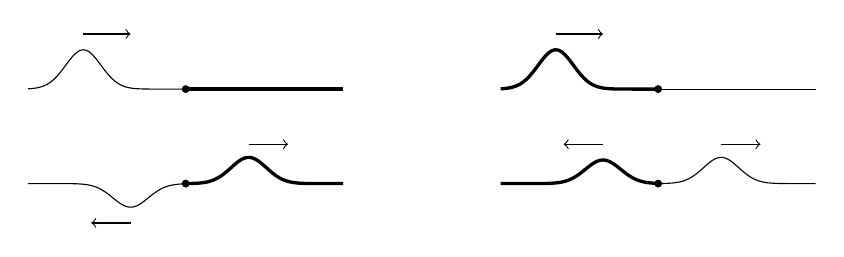
\begin{tikzpicture}
\begin{scope}[shift={(-3,0.6)}]
\path (0,0)--(0,0.78);
	\draw [samples=50, domain=-1:1, variable=\x] plot({\x},{exp(-(\x+0.3)*(\x+0.3)*10)/2});
	\fill (1,0) circle(0.05);
	\draw[very thick](1,0)--(3,0);
	\draw [->] (-0.3,0.7) -- +(0.6,0);
\end{scope}
\begin{scope}[shift={(-3,-0.6)}]
	\path (0,0) -- (0,-0.58);
	\draw [samples=50, domain=-1:1, variable=\x] plot({\x},{-0.6*exp(-(\x-0.3)*(\x-0.3)*10)/2});
	\draw [->] (0.3,-0.5) -- +(-0.5,0);
	\fill (1,0) circle(0.05);
	\draw[domain=1:3,samples=50, variable=\x, very thick] plot ({\x},{exp(-(\x-1.8)*(\x-1.8)*10)/3});
	\draw [->] (1.8,0.5) -- +(0.5,0);
\end{scope}

\begin{scope}[shift={(3,0.6)}]
	\draw [very thick,samples=50, domain=-1:1, variable=\x] plot({\x},{exp(-(\x+0.3)*(\x+0.3)*10)/2});
	\fill (1,0) circle(0.05);
	\draw(1,0)--(3,0);
	\draw [->] (-0.3,0.7) -- +(0.6,0);
\end{scope}
\begin{scope}[shift={(3,-0.6)}]
	\draw [very thick, samples=50, domain=-1:1, variable=\x] plot({\x},{0.6*exp(-(\x-0.3)*(\x-0.3)*10)/2});
	\draw [->] (0.3,0.5) -- +(-0.5,0);
	\fill (1,0) circle(0.05);
	\draw[domain=1:3,samples=50, variable=\x] plot ({\x},{exp(-(\x-1.8)*(\x-1.8)*10)/3});
	\draw [->] (1.8,0.5) -- +(0.5,0);
\end{scope}
\end{tikzpicture}
\caption{Reflexão e refração de ondas mecânicas numa corda esticada com dois
segmentos de densidades diferentes. À esquerda, a onda incidente propaga-se no
segmento menos denso e ocorre uma inversão de fase na onda refletida; à direita,
a onda incidente propaga-se no segmento mais denso e não há inversão de fase na
reflexão. A onda refratada não sofre variação de fase em qualquer dos
casos.\label{fig:40-060}}

}
\end{figure}

Em resumo, a variação de fase sofrida por uma onda de luz no processo de
reflexão é dada por
\begin{equation*}
\delta\varphi_r = 
\begin{cases}
    0&\text{se } n_1>n_2\\
    \pi&\text{se } n_1<n_2,
\end{cases}
\end{equation*}
onde $n_1$ é o índice de refração do meio onde a luz incidente se propaga e
$n_2$ é o do meio contra o qual a luz incide.


\subsection*{Alterações de fase na refração}
Aqui, a situação é mais simples: nos processos de refração nunca ocorre qualquer
variação de fase da onda. Isso mesmo é de certa forma também ilustrado na
Figura~\ref{fig:40-060}, onde se pode ver que a fase da onda refratada é, nas
duas situações representadas, igual à da onda incidente.

\subsection*{Alterações de fase na propagação}
Vimos já, na Secção~\ref{sec:dfidx}, que a variação de fase de uma onda
monocromática com comprimento de onda $\lambda$ em dois pontos do seu percurso
separados por uma distância $d$ é dada por
\begin{equation*}
    \delta\varphi_p=2\pi\frac{d}{\lambda}.
\end{equation*}
Podemos pois usar esta fórmula para calcular as variações de fase sofridas pela
onda que se reflete na superfície posterior da película devidas ao trajeto de
ida e de volta até à superfície incidente. É necessário apenas notar que no
interior da película o comprimento de onda da luz tem um valor inferior ao que
apresenta no vácuo, pois a luz desloca-se no interior da película mais devagar.
Um pouco de reflexão mostra que o valor do comprimento de onda no interior da
película é $\lambda/n_p$, onde $\lambda$ representa o comprimento de onda no
vácuo e $n_p$ o índice de refração do material que constitui a película. Com
este valor alterado do comprimento de onda, a variação de fase nos dois
trajetos (de ida e no regresso) vem dada por
\begin{equation*}
\delta\varphi_p=2\times2\pi n_p\frac{s}{\lambda},
\end{equation*}
onde o factor 2 se deve ao facto de a espessura da película, $s$, ser percorrida
duas vezes (uma à ida, a outra no regresso).
\begin{center}
    \rule{2cm}{0.1mm}
\end{center}

Agora que estabelecemos expressões para o cálculo de todas as variações de fase
sofridas por cada raio, podemos calcular afase de cada um quando se recombinam
e, mais importante, podemos calcular a diferença de fase com que se sobrepõem.
Assim, podemos determinar em que condições é que essa sobreposição é construtiva
ou destrutiva.

Vejamos um exemplo. As bolas de sabão com que as crianças brincam apresentam
frequentemente reflexos coloridos e, por vezes, têm zonas que se tornam
invisíveis (normalmente no lado de cima), por não se verem nelas quaisquer
reflexos. Qual deve ser a menor espessura da película de água e sabão (com
índice de refração $n=1,33$) para a qual se anula o reflexo de um raio de luz
com comprimento de onda 520\,nm, incidindo perpendicularmente na película?

Seja $\varphi_0$ a fase do raio incidente no ponto de incidência e num dado
instante e $\varphi_1$ e $\varphi_2$ as fases dos dois raios refletidos
($\varphi_1$ a do raio que reflete na face de incidência, $\varphi_2$ a do que
se reflete na face oposta) nesse instante nos pontos em que abandonam a
película. De acordo com o referido acima sobre as variações de fase que ocorrem
nas reflexões, tendo em conta que o índice de refração da película (água com
sabão) é maior do que o do ar, concluímos que 
\begin{equation*}
\varphi_1=\varphi_0+\pi.
\end{equation*}
Já o raio que se reflete na face oposta aquela onde se dá a incidência não sofre
qualquer variação de fase na reflexão, uma vez que ela se faz contra um meio
(ar) com um índice de refração inferior ao daquele onde a luz se propaga
(película). Assim, e porque não há quaisqer variações de fase nas refrações, a
fase deste raio varia apenas devido à propagação do raio no atravessar da
película nos dois sentidos. Podemos então escrever
\begin{equation*}
\varphi_2= \varphi_0+4\pi n\frac{s}{\lambda},
\end{equation*}
onde $s$ é a espessura da película e $n=1,33$ é o índice de refração da água com
sabão. A diferença de fase entre os dois raios é então
\begin{equation*}
\delta\varphi = \varphi_2-\varphi_1=4\pi n\frac{s}{\lambda}-\pi
\end{equation*}
Pretende-se determinar o menor valor de $s$ para o qual se anula o reflexo do
raio incidente, ou seja para o qual a interferência dos dois raios refletidos é
destrutiva. Mas sabemos já que esta interferência é destrutiva se
$\delta\varphi=(2k+1)\pi$, com $k=0,\pm1,\pm2,\ldots$. Então,
\begin{align*}
4\pi n\frac{s}{\lambda}-\pi&=(2k+1)\pi\\
s&=\frac{k+1}{2n}\lambda.
\end{align*}
O menor valor de $s$ (ainda positivo, é claro) obtém-se nesta fórmula tomando
$k=0$, resultando $s=\lambda/2n\simeq 195$\,nm.

\newpage
\section*{Interferência --- Resumo}
\tobedone{}
\begin{itemize}[leftmargin=*]
  \item
\end{itemize}
